\chapter{Experiments and Results}
\label{AER}

In the following section I will apply the software to demonstrate the predicted dynamics of the phages and bacteria under different conditions. 
I first begin with analyzing the model using a SOBOL analysis on the simple Golding model, \Cref{eq:golding_model}. 
Using the most important parameters identified from the SOBOL analysis, I run multiple IVAs to describe the change in graph behavior for different inputs. 
I use the information gained from this to describe how the graphs change for a wide range of inputs. 
Next, I analyze if phages will proliferate or not depending on the initial phage, uninfected bacteria, and resource concentration. 
I finally extend the analyses to a large community and analyze how changing parameter values will change the phage and bacteria growth, and if the phages and bacteria can coexist or not. 

\section{SOBOL Sensitivity Analysis Results}
\label{sec:SOBOL_sensitivity_analysis_results}
The SOBOL method is a global sensitivity analysis technique that quantifies the contribution of each input parameter, as well as their interactions, to the variance of a model's univariate output. 
It decomposes the output variance into fractions attributed to individual parameters and their combinations, providing first-order and total-order sensitivity indices.
A SOBOL analysis identifies the most influential parameters affecting model output. 
The insights from this analysis inform the selection of key parameters for subsequent simulations, ensuring that further investigations focus on those with the greatest impact.

\Cref{fig:created:SOBOL_final_no_wi_wo} shows the impact that the parameter had on the final value of the population at $t=15$ for a $1\times 1\times 1$ system, on the original Golding model, \Cref{eq:golding_model}. 
\Cref{fig:created:SOBOL_peak_no_wi_wo} shows the impact that the parameter had on the peak population count, using the 95\% rule. 
\Cref{fig:created:SOBOL_peak_time_no_wi_wo} shows the impact that the parameter had on the time of the peak, using the 95\% rule. 

The parameters that were tested include all the parameters listed in the basic Golding model, except for the uninfected bacteria $(I_1, \dots, I_4), M, \omega^i,$ and $\omega^o$. 
Infected bacteria was not included as it doesn't make sense to start with infected bacteria to the system. 
$M$, the number of stages that the infection goes through, can not be tested as SOBOL as $M$ is an integer, while SOBOL randomly chooses float values. 
While testing, the washin rate $\omega^i$ and washout rate $\omega^o$ consistently had the largest influence on the final, peak value, and time of peak value, using the 95\% rule. 
Washin and washout are not part of the original model from Golding, and the addition of a washin and washout term significantly skews the results and analysis, so it was left out of the analysis. 
The results for a SOBOL analysis with washin and washout can be found in \Cref{sec:AppendixF:sobol_analysis_with_washin_and_washout}. 

\subsection{Resources}
The final value for the resources depended heavily on the initial resource concentration. 
There weren't many interactions with other parameters because $ST \gg S1$. 
$e$ had little influence on the system despite $e$ acting as the link between the resources and bacteria and directly controlling the rate of resource consumption. 
$\tau$ had a larger influence in the final resource value than $e$. 

The peak value and time of peak value graphs are empty for the SOBOL indices for Resources as the resource concentration is always decreasing from different initial conditions, the initial resource always had a peak at $t=0$. 

\subsection{Phages}
The final phage population value depended on $r$ the most, with $\beta$ as the second most important parameter influencing the final population value. 
The other parameters had little to no influence on the final phage population levels. 

The SOBOL peak value plot is basically the same as the final population value. 
Similar to the final value, the phage max value is highly dependent on the value of $r$ and $\beta$, and the other parameters had little to no influence on the peak value for the phages. 

For the time of peak value, $\tau$ becomes the most important parameter for determining the time of peak value, while $r$ isn't as important anymore. 
The initial phage population has a small influence on the final population value, about as equally important as $r$. 
$\beta$ roughly maintains the same sensitivity value across the final, peak, and time of peak analyses. 

\subsection{Total Bacteria}
The final total bacteria population depended mostly on $\beta$, the burst size of the phage, but via many second or there are many higher order interactions occurring as $ST \gg S1$. 
The final population depended heavily on many higher order interactions with the initial resource concentration, $\tau$, and $e$. 

$\beta$ is still the most important parameter to the model, but instead of $ST$ and $S1$ being equal to 1 and 0.28 like in the final value, the sensitivity value is only 0.54 and 0.16 respectively. 
Every parameter plays some influence on the output, but with higher order interactions as for all parameter inputs, $ST > S1$. 

$\beta$ and $\tau$ are the two most important factors in determining the time of peak for the total bacteria. 
The only parameter that does not influence the time of peak in some manner is $e$, otherwise every parameter has some sort of influence on the time at which the bacteria population peaks. 

\subsection{Results}
Some results are surprising. 
$e$, $v$, and $K$ are consistently the least important factor in determining the final value, peak value, and time of peak. 
It would be expected that changing the parameter values that directly affect the bacterial growth would have a large impact on the resources and phages. 
More bacteria mean more resources are consumed, and more phages are created. 
Knowing that $e$, $v$, and $K$ are relatively unimportant compared to a parameter like $r$ or $\tau$, future analyses do not have to focus on $e$, $v$, and $K$. 
As $\beta$, $r$, and $\tau$ are relatively important, future analyses could focus on how those parameters influence the growth of phages and bacteria. 


\begin{figure}[ht!]
    \centering
    \begin{subfigure}{0.32\linewidth}
        \centering
        \captionsetup{width=1\linewidth}
        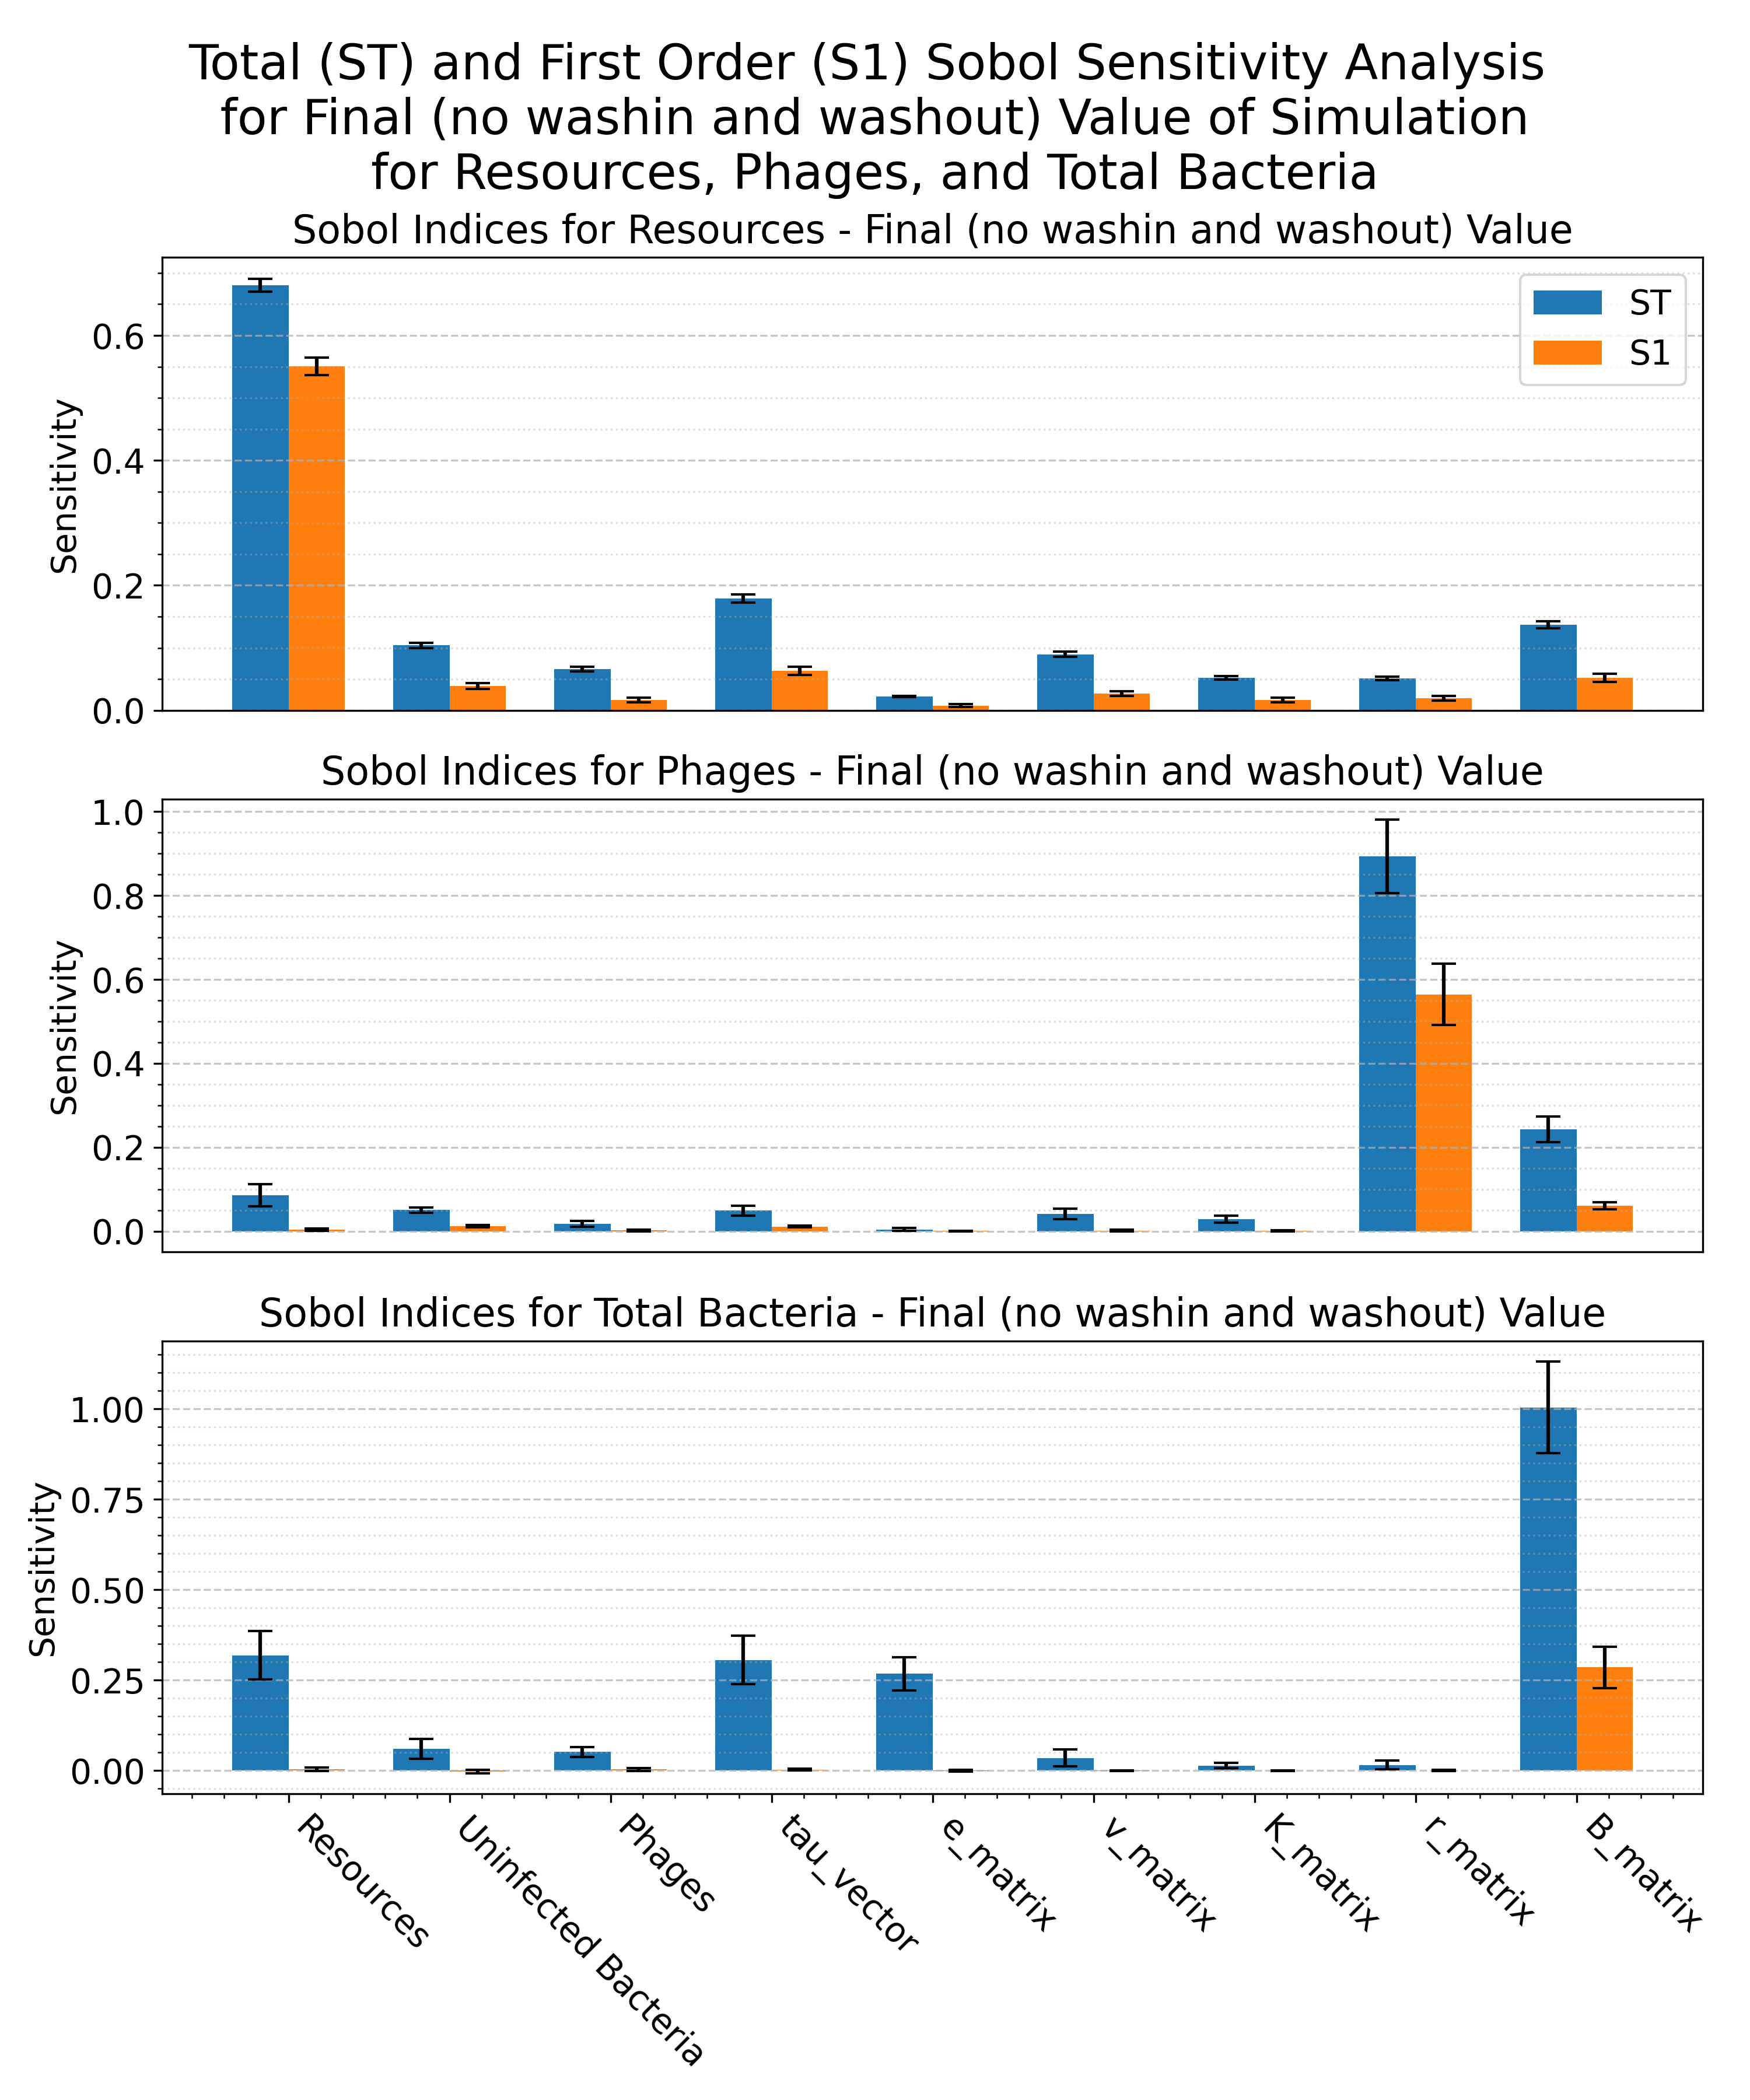
\includegraphics[width=\linewidth]{Plots/Created/SOBOL/SOBOL_analysis_1749708738_Final_(no_washin_and_washout).png}
        \caption{
            Final value, no washin and washout. 
        }
        \label{fig:created:SOBOL_final_no_wi_wo}
    \end{subfigure}
    \hfill
    \begin{subfigure}{0.32\linewidth}
        \centering
        \captionsetup{width=1\linewidth}
        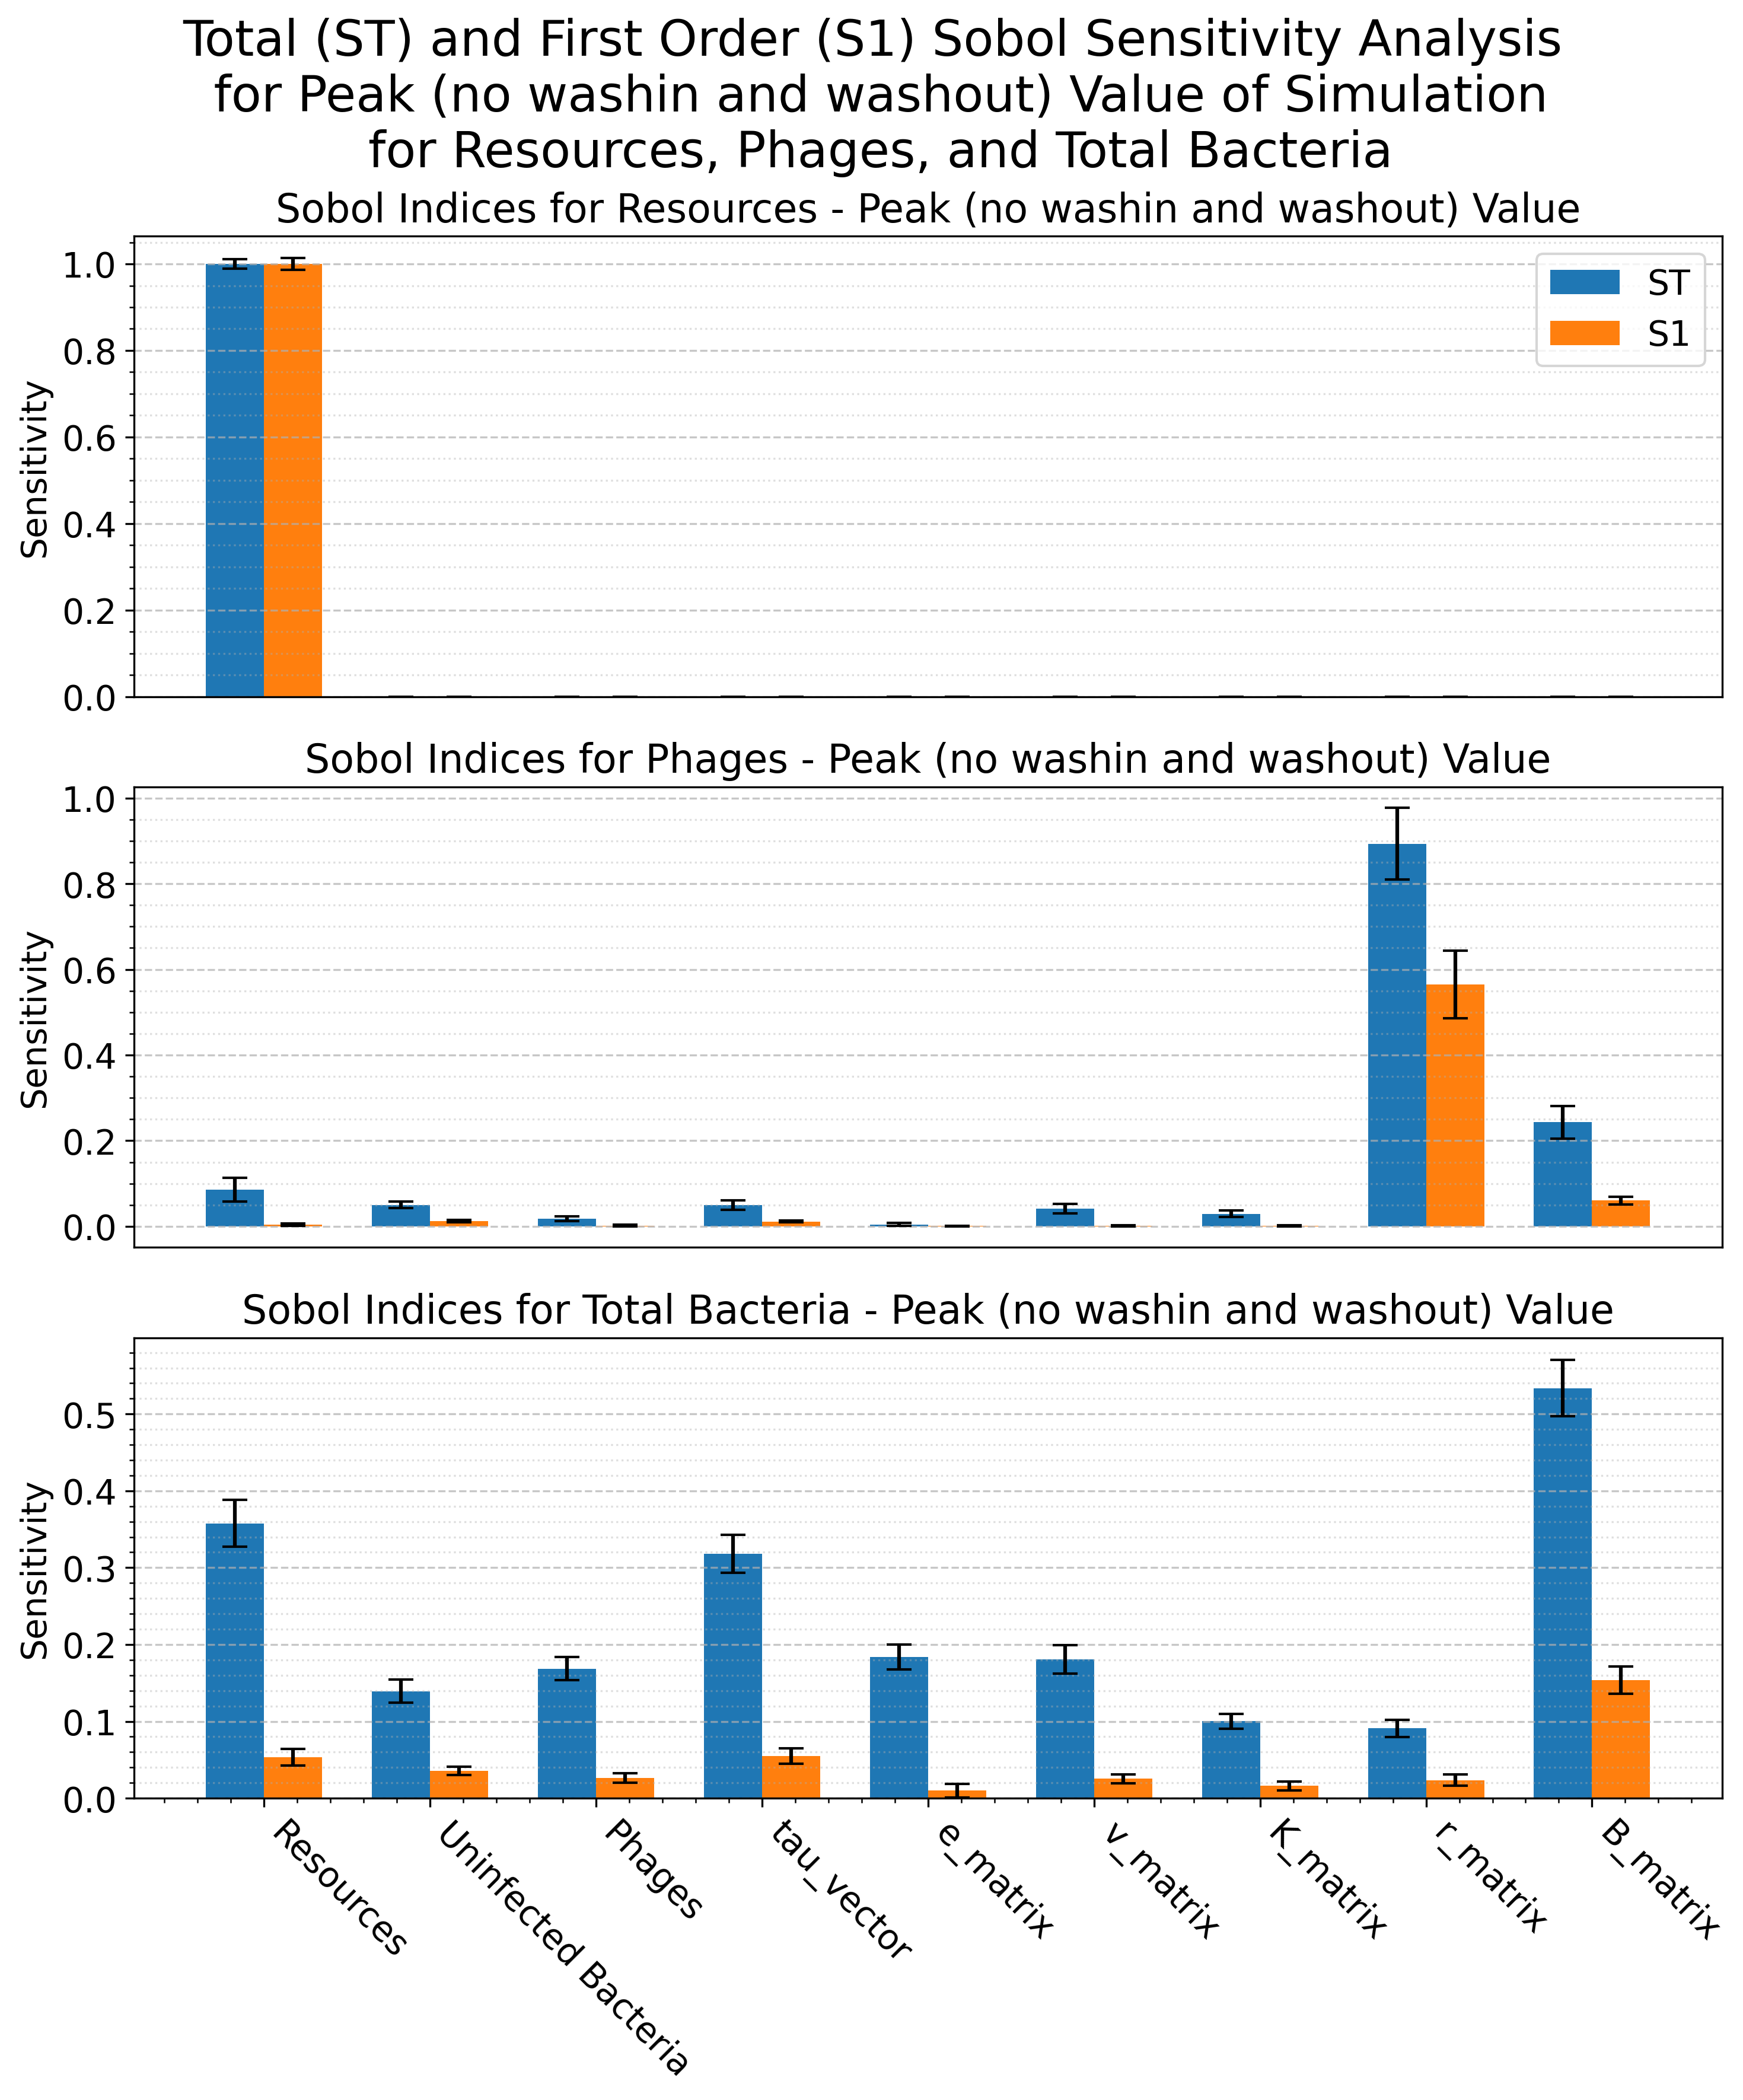
\includegraphics[width=\linewidth]{Plots/Created/SOBOL/SOBOL_analysis_1749708738_Peak_(no_washin_and_washout).png}
        \caption{
            Peak population value, no washin and washout. 
        }
        \label{fig:created:SOBOL_peak_no_wi_wo}
    \end{subfigure}
    \hfill
    \begin{subfigure}{0.32\linewidth}
        \centering
        \captionsetup{width=1\linewidth}
        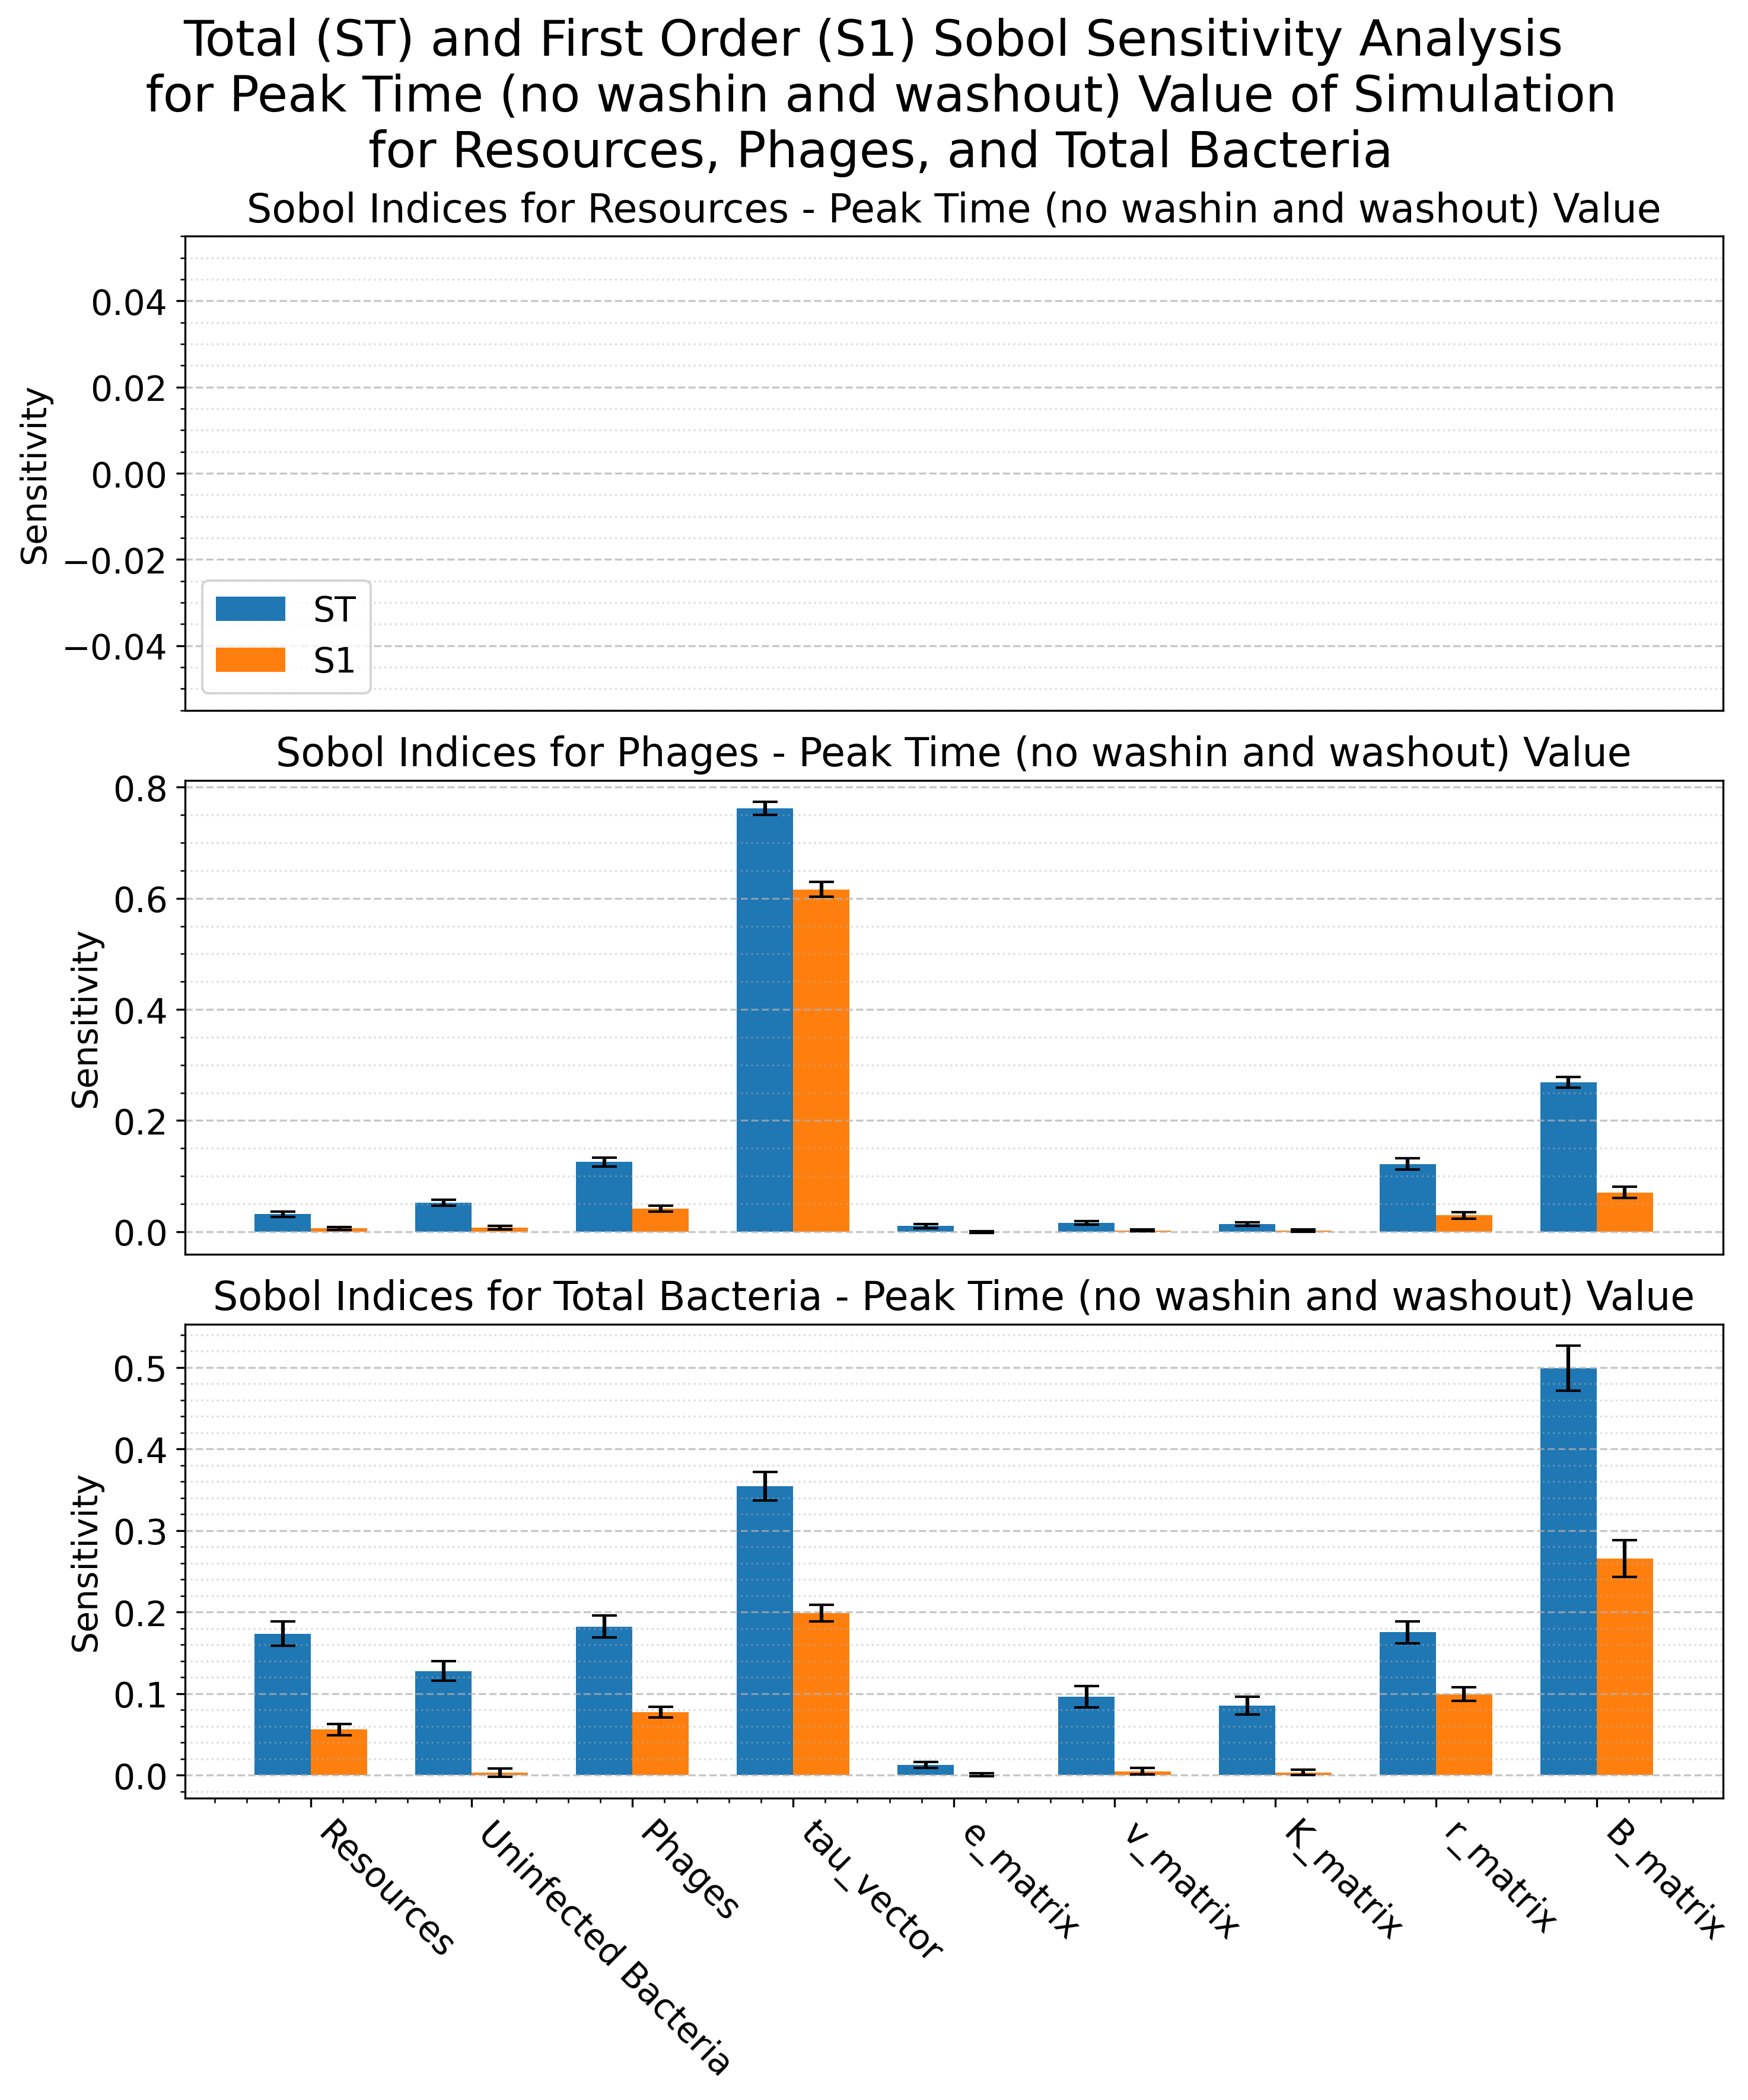
\includegraphics[width=\linewidth]{Plots/Created/SOBOL/SOBOL_analysis_1749708738_Peak_Time_(no_washin_and_washout).png}
        \caption{
            Time of peak value, no washin and washout. 
        }
        \label{fig:created:SOBOL_peak_time_no_wi_wo}
    \end{subfigure}
    \caption{
        SOBOL analyses for the final, peak, and time of peak value, without a washin and washout rate.
        The input value ranges to test each parameter used for this SOBOL test can be found in \Cref{tab:appendixE:SOBOL_analysis_values}, except washin and washout is 0. 
    }
    \label{fig:created:SOBOL_no_wi_wo}
\end{figure}

\section{Graph Behavior with IVA}
\Cref{fig:created:a_good_curve_linear} is used as a “ground truth” for what a researcher would aim to replicate in a lab.  
\Cref{tab:results:graph_behavior} quantitatively elaborates how a change in parameter value across multiple values changes the shape of the population curves. 
Only the most important parameters identified in the SOBOL section, will be analyzed, so initial resource concentration, $\tau$, $r$, and $\beta$. 

\begin{table}
    \footnotesize
    \centering
    \begin{tabularx}{\textwidth}{l l X}
        \toprule
        \textbf{Parameter} & \textbf{Tested Value} & \textbf{Behavior Description} \\
        \midrule
        $R$ (400) & 500 & More uninfected and infected bacteria, slightly more phages. Resources last longer before being depleted. \\
         & 300 & Slightly less uninfected and infected bacteria, slightly less phages, and earlier resource depletion. \\

        \midrule
        $U$ (50) & 70 & Slightly more phages and uninfected and infected bacteria. Resources are depleted faster. \\
         & 30 & Less uninfected and infected bacteria, slower resource depletion, not all resources used, slightly less phages are created. \\

        \midrule
        $P$ (10) & 20 & Less resources consumed, less bacteria created, bacteria population peaks earlier, slightly less phages.\\
         & 5 & Resources are consumed faster, more uninfected, infected, and phages. Bacteria population peaks at a later time. \\

        \midrule
        $\tau$ (2.14) & 3 & Bacteria population peaks later, with a plateau in population after peaking before infections take place. Phages population is still growing. Infected bacteria peak significantly later. Significant increase in bacteria population. \\
         & 0.5& Barely any resource consumption, little bacteria growth and uninfected, more phages created, phages reach final value very fast. Bacteria population peaks very early. \\

        \midrule
        $\omega^i$ (0) & 15 & Slightly more bacteria are created, resource replenish after bacteria die out. Resources are not depleted and regrow after bacteria die out. Slightly more bacteria are created. \\

        \midrule
        $e$ (0.03) & 0.1 & Faster resource depletion, sharper decline in uninfected, slightly less infected bacteria and phages. Drop in uninfected bacteria happens faster. Bacteria sum peak is sharper and happens earlier. \\
         & 0.01 & Not all resources are consumed, slightly more bacteria are created. \\

        \midrule
        $v$ (1.2) & 1.8 & Resources are finished faster, significantly more uninfected and infected bacteria. Bacteria population peaks earlier, and there are more phages. Peak of the bacteria curve is more sharp and less rounded. \\
         & 1 & Less phages and bacteria are created, not all resources are consumed, bacteria population peaks a tiny bit earlier.\\

        \midrule
        $K$ (10) & 500 & Not all resources are consumed, less bacteria and phages are created, earlier bacteria peak.\\
         & 1 & Faster resource depletion and sudden stop instead of gradual slowdown, more uninfected, infected, and phages create. \\

        \midrule
        $r$ (0.01) & 0.1 0.1& Less resource consumption, significantly less bacteria and phages, earlier peak in bacteria.\\
         & 0.001 & Faster resource consumption rate, significantly more bacteria and phages, delay in uninfected and infected peak, sharp uninfected bacteria peak, sharp bacteria sum peak with a mini plateau before dropping. \\

        \midrule
        $\beta$ (20) & 50 & Significantly more phages and significantly less bacteria, earlier bacteria peak, less resources consumed. Steeper fall in uninfected bacteria, steeper rise in infected bacteria. \\
         & 10 & Faster resource consumption, significantly more uninfected, less phages, sharper uninfected and total bacteria peak, total bacteria population has a plateau before falling. \\

        \midrule
        $\omega^o$ (0) & 0.02 & Faster resource depletion, more bacteria created, later peak in bacteria population. Faster decrease in uninfected bacteria, slightly less phages created, with a gradual decrease in phages post peak. \\

        \bottomrule
    \end{tabularx}
    \caption{
        A table that compares how moving one individual parameter value up or down relative to \Cref{fig:created:a_good_curve_linear} changes the general shape of the curve. 
        Reference parameter values used to compare the produced curves are included in the parentheses, taken from \Cref{tab:appendixE:a_good_curve}. 
    }
    \label{tab:results:graph_behavior}
\end{table}

\section{Initial Value Analysis Results}
\label{sec:results:initial_value_analysis}

\Cref{fig:created:initial_value_analysis_UB_50_500_a_good_plot_2} and \Cref{fig:created:initial_value_analysis_UB_50_500_a_good_plot} illustrate how varying the initial uninfected bacteria population from 1 to 500 (using 100 different starting values) affects the dynamics and time of peak population of phage and total bacteria populations using the 95\% rule. 

\Cref{fig:created:initial_value_analysis_UB_50_500_a_good_plot_2} perfectly replicates Figure 1 of \citet{mullaExtremeDiversityPhage2024}. 
As the initial bacteria population increases, the time to reach the phage and bacteria sum peak decreases, following $y = -0.8648\cdot ln(x) + 9.7911$ and $y = -1.0056\cdot ln(x)+7.7626$, with $R^2=0.9800, 0.9988$ respectively. 

\Cref{fig:created:initial_value_analysis_UB_50_500_a_good_plot} on the other hand shows different behavior. 
As the initial bacteria population decreases from 500 to 100, \Cref{fig:created:initial_value_analysis_UB_50_500_a_good_plot_2} exhibits the same behavior. 
There is a change in behavior at 100 and less initial uninfected bacteria. 
Instead of following the predicted line like in \Cref{fig:created:initial_value_analysis_UB_50_500_a_good_plot_2}, the curve for the phages suddenly decreases, following a non-monotonic curve. 
The bacteria on the other hand plateau before starting to increase again. 
The fitted curves follow $y = -0.1292\cdot ln(x) + 10.1462$ and $y = -0.6234\cdot ln(x)+6.9602$, with $R^2=0.5406, 0.9206$ respectively. 
The slope tells us how well the uninfected bacteria has an influence on the time of peak value. 
The larger (positive or negative) the slope is, the more impact the uninfected bacteria had on the time of peak value. 
The closer the $R^2$ value is to 1, the more proportion of the variance for the time to peak value is explained by the uninfected bacteria. 
There is a deviation because the model changes limiting regions. 

\begin{figure}
    \centering
    \begin{subfigure}{1\linewidth}
        \centering
        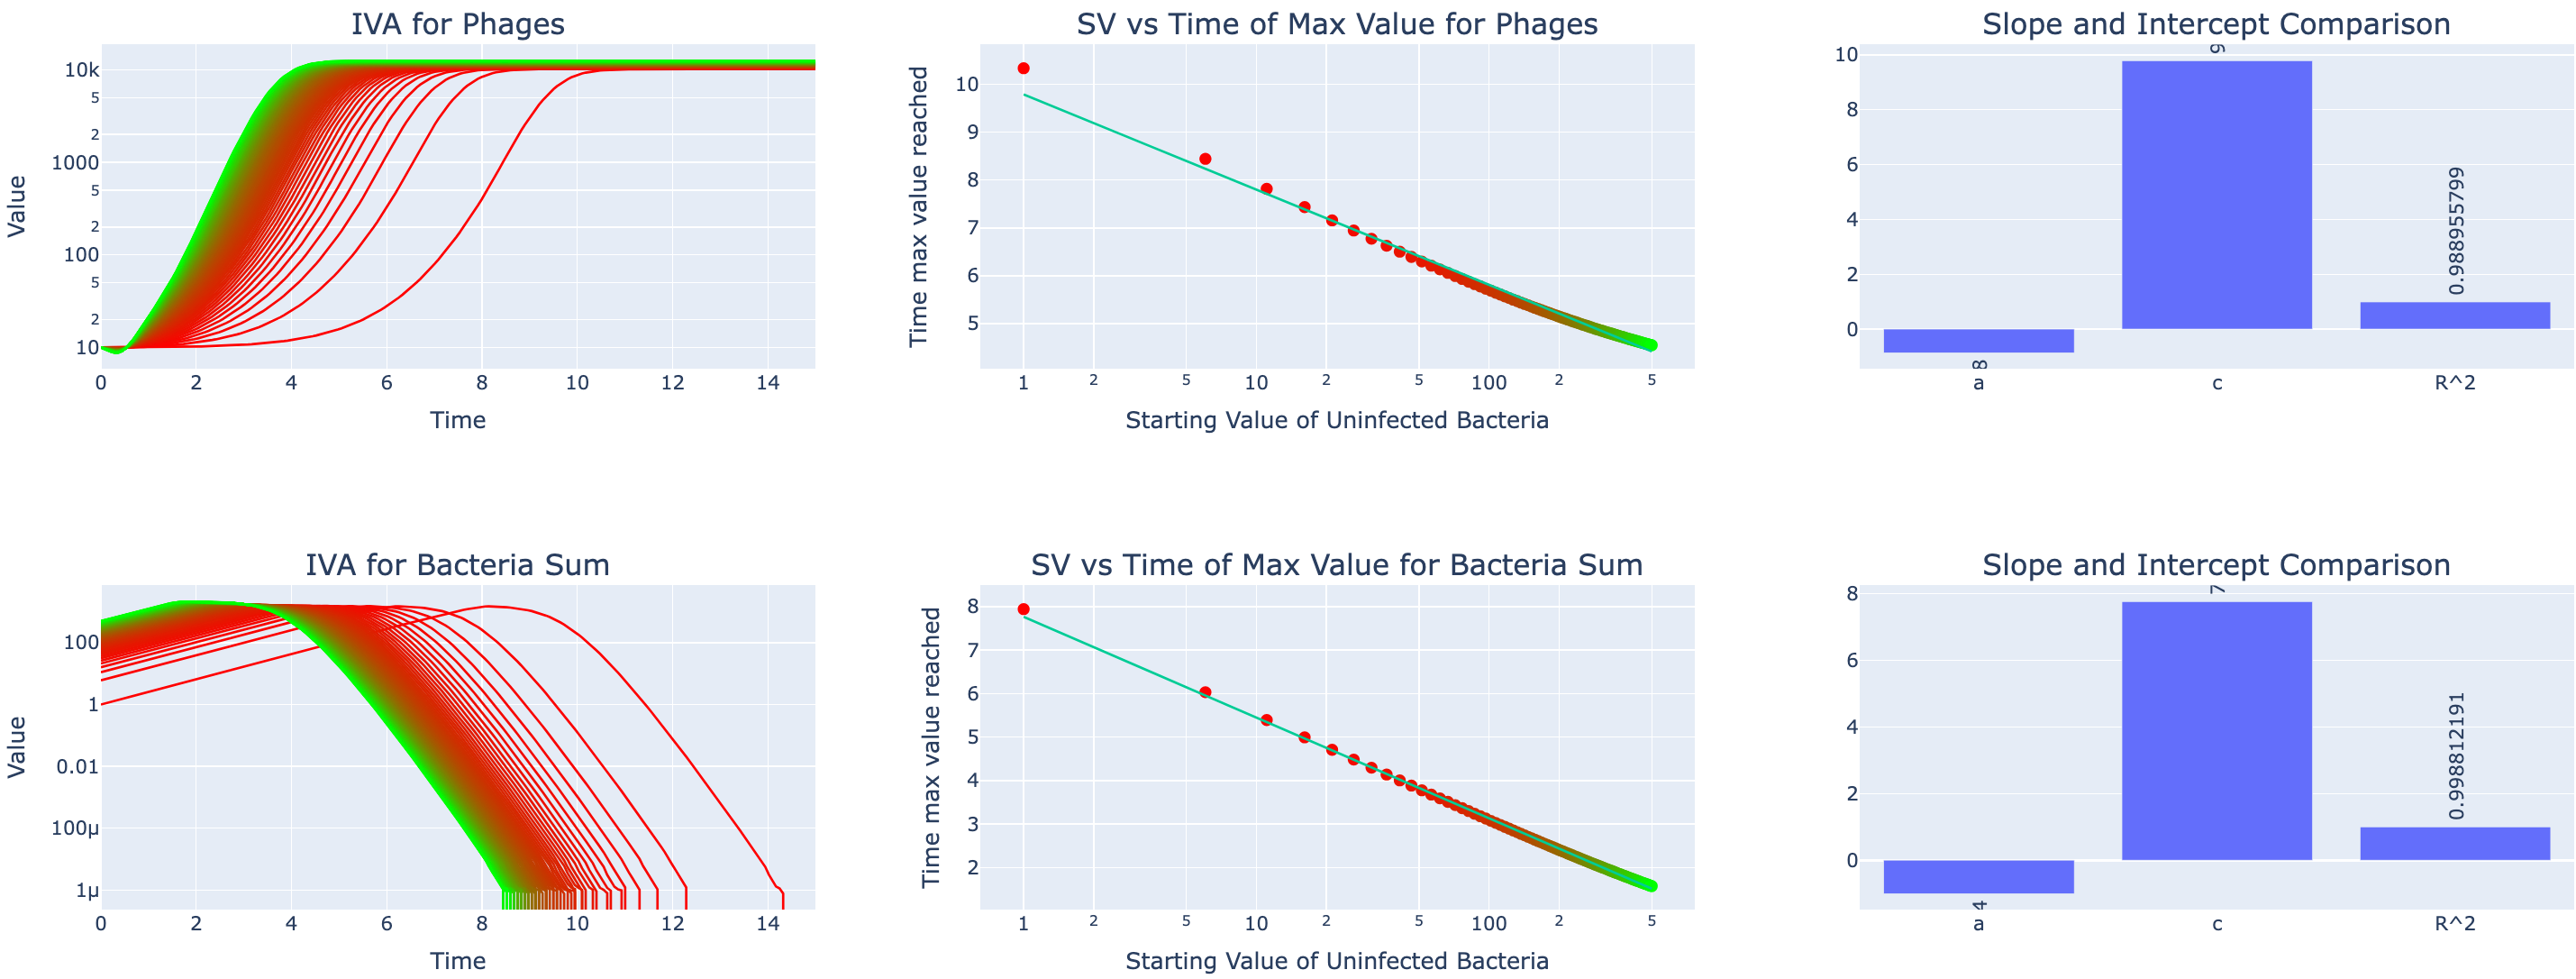
\includegraphics[width=\linewidth]{Plots/Created/IVA/initial_value_analysis_UB_50_500_a_good_plot_2.png}
        \caption{
            IVA for \Cref{tab:appendixE:a_good_curve_2}. 
            Replicates Figure 1 of \citet{mullaExtremeDiversityPhage2024}. 
            The system is adsorption limited \cite{mullaExtremeDiversityPhage2024}. 
        }
        \label{fig:created:initial_value_analysis_UB_50_500_a_good_plot_2}
    \end{subfigure}
    \hfill
    \begin{subfigure}{1\linewidth}
        \centering
        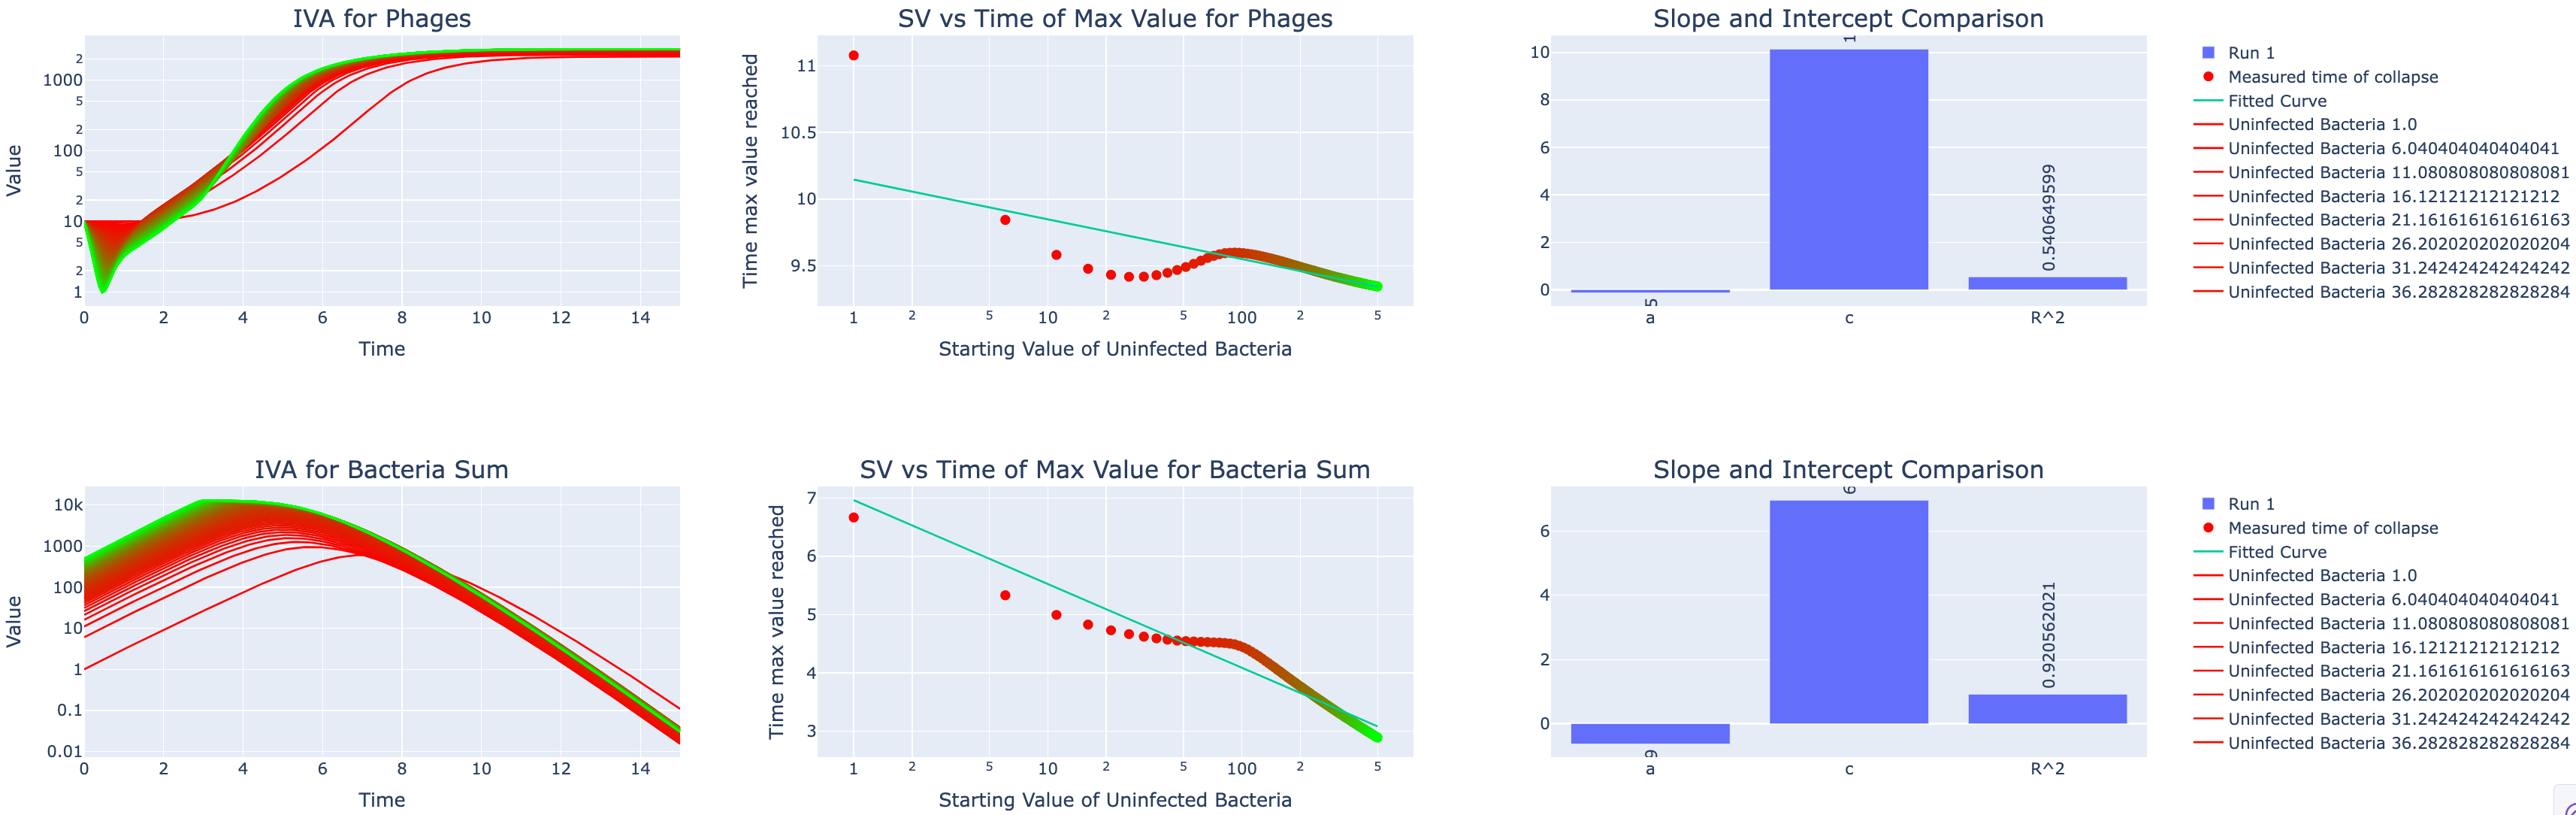
\includegraphics[width=\linewidth]{Plots/Created/IVA/initial_value_analysis_UB_50_500_a_good_plot.png}
        \caption{
            IVA for \Cref{tab:appendixE:a_good_curve}. 
            For uninfected bacteria less than 100, the phage-bacteria interaction is resource limited. 
        }
        \label{fig:created:initial_value_analysis_UB_50_500_a_good_plot}
    \end{subfigure}
    \caption{
        Varying the initial uninfected bacteria concentration, from 50 to 500, with 30 unique values tested. 
        Varying the default parameter values a can have a large influence on how changing the initial bacteria concentration influences the dynamics of the system. 
        The default values for Figure a) and b) can be found at \Cref{tab:appendixE:a_good_curve} and \Cref{tab:appendixE:a_good_curve_2}. 
    }
\end{figure}

\section{Phage Proliferation}
\label{sec:results:phase_portrait}
\subsection{Phase Portrait}
\Cref{fig:created:phase_portrait_resources_245-265_phages_25-26} shows a phase portrait varying the initial resource and phage concentration. 
The same initial phage values have the same color for the line. 
For phages that start above 25.98, the phage population can proliferate until the washout would eventually remove the phages. 
For phage populations that start below 25.98, the washout removes the phages before the phages had time to infect and kill the bacteria. 
Both regions of phages exhibit consistent behavior, of either going to 0 or proliferating. 
If the phage population started at exactly 25.98, if the initial resources was 260 or above, the phages died out. 
If the initial resource value was 255 or below, the phages proliferated. 

\subsection{An Initial Phage and Resource Analysis for Phage Proliferation}
\Cref{fig:created:phase_portrait_resources_phage} expands on the phase portrait by simulating more values and coloring the square depending on if the phages proliferated or not. 
The initial resource values span from 1 to 500, and the initial phage values range from 25.5 to 26.5, each with 100 unique values sampled.
A boundary between the non-proliferating and proliferating phages can be curve-fit following $y=\frac{86.756x}{15.811+x} - 10.241$ with an $R^2$ value of 0.994. 

\Cref{fig:created:phase_portrait_resource_phage_proliferate} zooms into the range $(1-40, 24.2-25)$ for a high detailed view of the behavior happening around initial resources of 10. 
From 1 to around 7 initial resources, fewer phages are needed to proliferate. 
At 7 initial resources, there is a minimum in the phage proliferation boundary. 
From 7 initial resources and upwards, as more resources are added to the system, more phages are needed to ensure proliferation. 
Despite this, the change is tiny, a difference of about 2 phages. 
Considering the range of possible initial phage populations, the phage proliferation boundary is essentially flat. 
Under these parameter values, choosing an initial phage population of 27 or higher will ensure phage proliferation. 
This behavior is counter-intuitive. 
It would be expected that as there are more resources, the bacteria would have more resources to consume, allowing more phages to grow. 
A reason for this behavior might be because as there are more resources, bacteria can grow faster. 
The bacteria growth population outpaces the growth rate of the phages, causing the phages to die out due to the washout. 

If there is a higher washout, similar behavior is observed where the phage proliferation boundary exhibits a similar shape to that of \Cref{fig:created:phase_portrait_resources_phage}, except more phages are needed to proliferate. 
If $K$ is increased to a larger value, the minimum in the proliferation boundary is shifted to the right. 

\begin{figure}[]
    \centering
    \begin{subfigure}{0.49\linewidth}
        \centering
        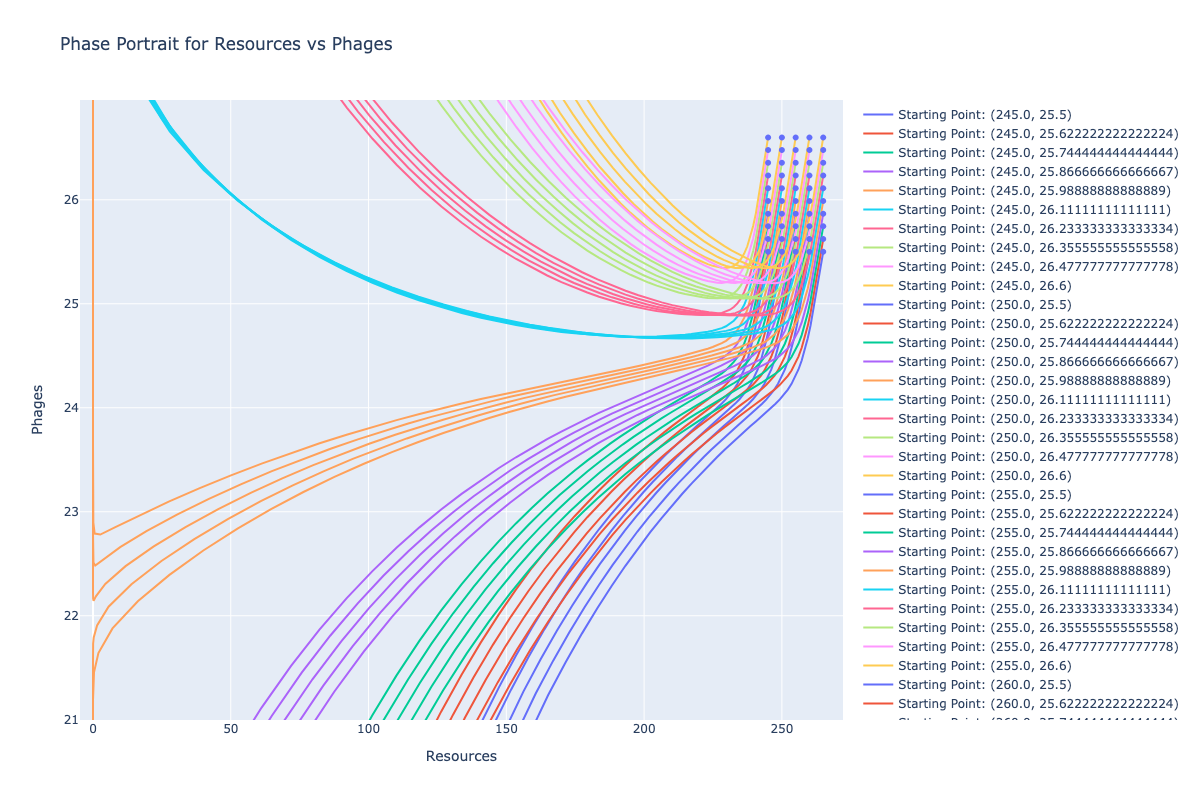
\includegraphics[width=1\textwidth]{Plots/Created/PP/phase_portrait_resources_245-265_phages_25-26.png}
        \caption{
            Zoomed in plot of a phase portrait with varying resource and phage population from 245-265 and 25.5-26.5 respectively. 
            Each row has its own line color. 
            Diverging behavior can be seen for the orange line (phage=25.98). 
        }
        \label{fig:created:phase_portrait_resources_245-265_phages_25-26}
    \end{subfigure}
    \hfill
    \begin{subfigure}{0.49\linewidth}
        \centering
        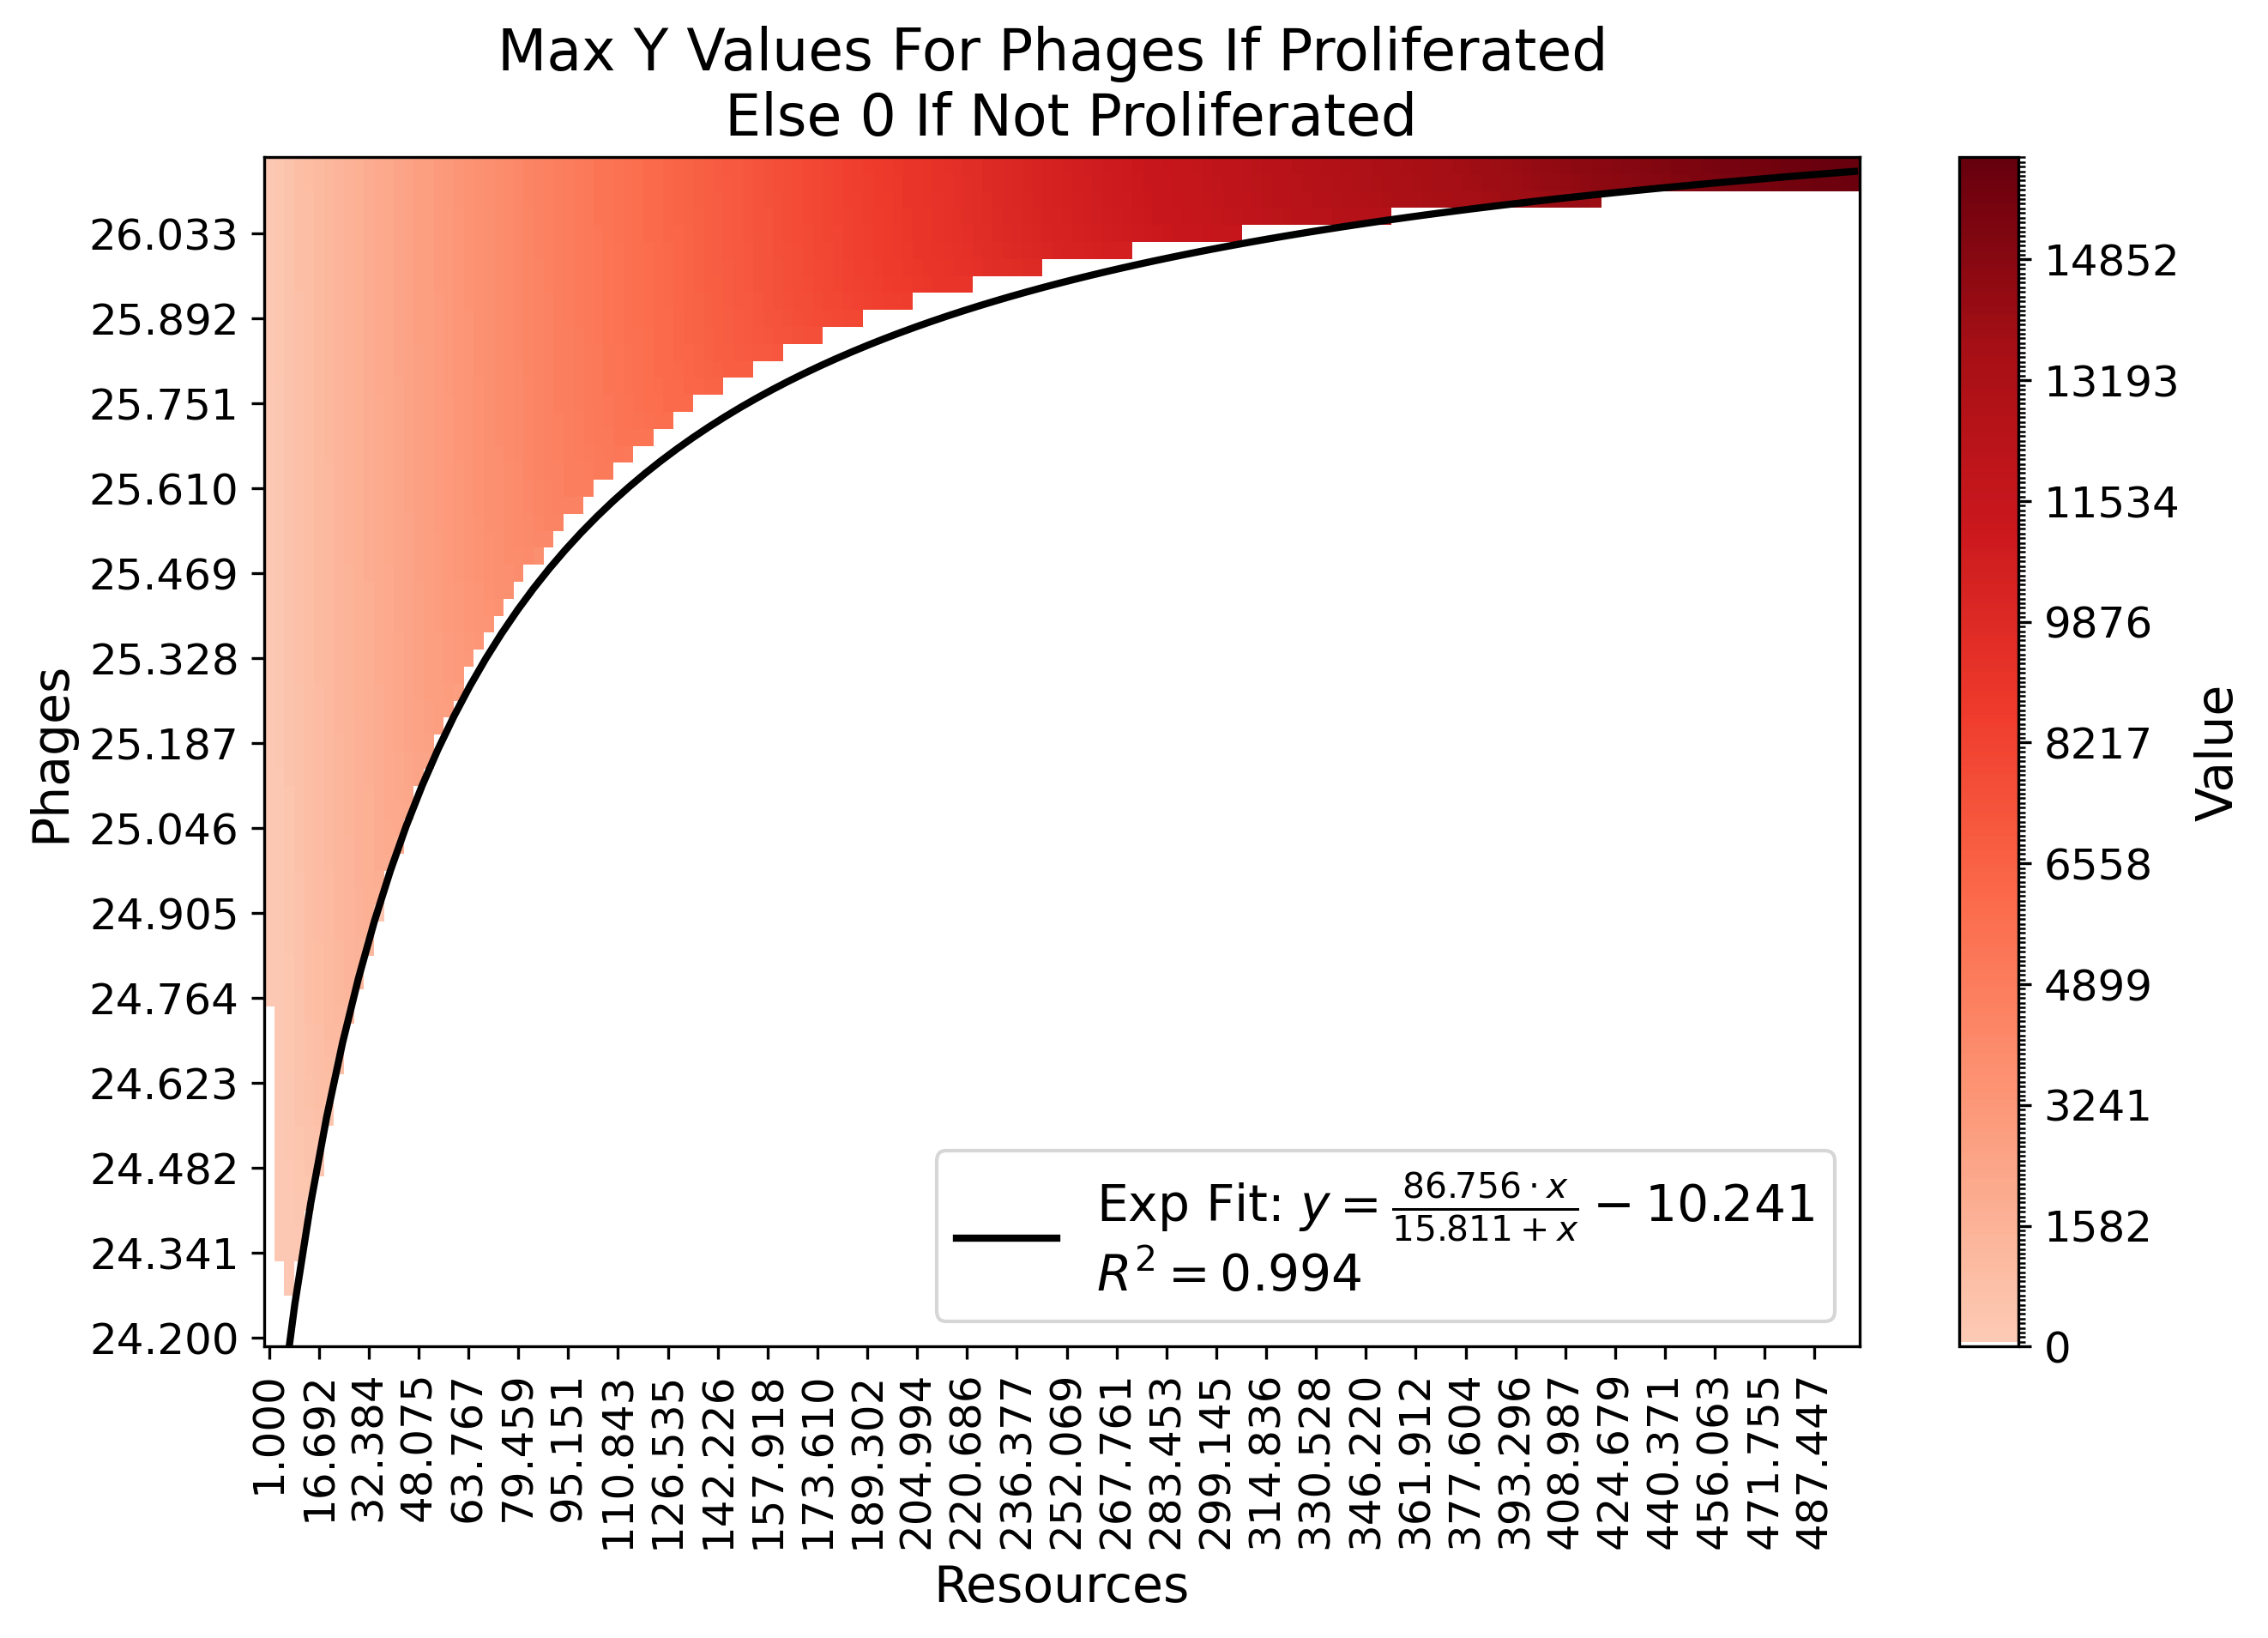
\includegraphics[width=\linewidth]{Plots/Created/PP/phase_portrait_resources_phage.png}
        \caption{
            Phage population proliferation as a function of initial resource and phage concentrations. 
            While the color appears uniform along the vertical axis, each cell is actually a slightly different value. 
            The phage-resource proliferation boundary follows a fitted Monod equation.
        }
        \label{fig:created:phase_portrait_resources_phage}
    \end{subfigure}
    \hfill
    \begin{subfigure}{0.49\linewidth}
        \centering
        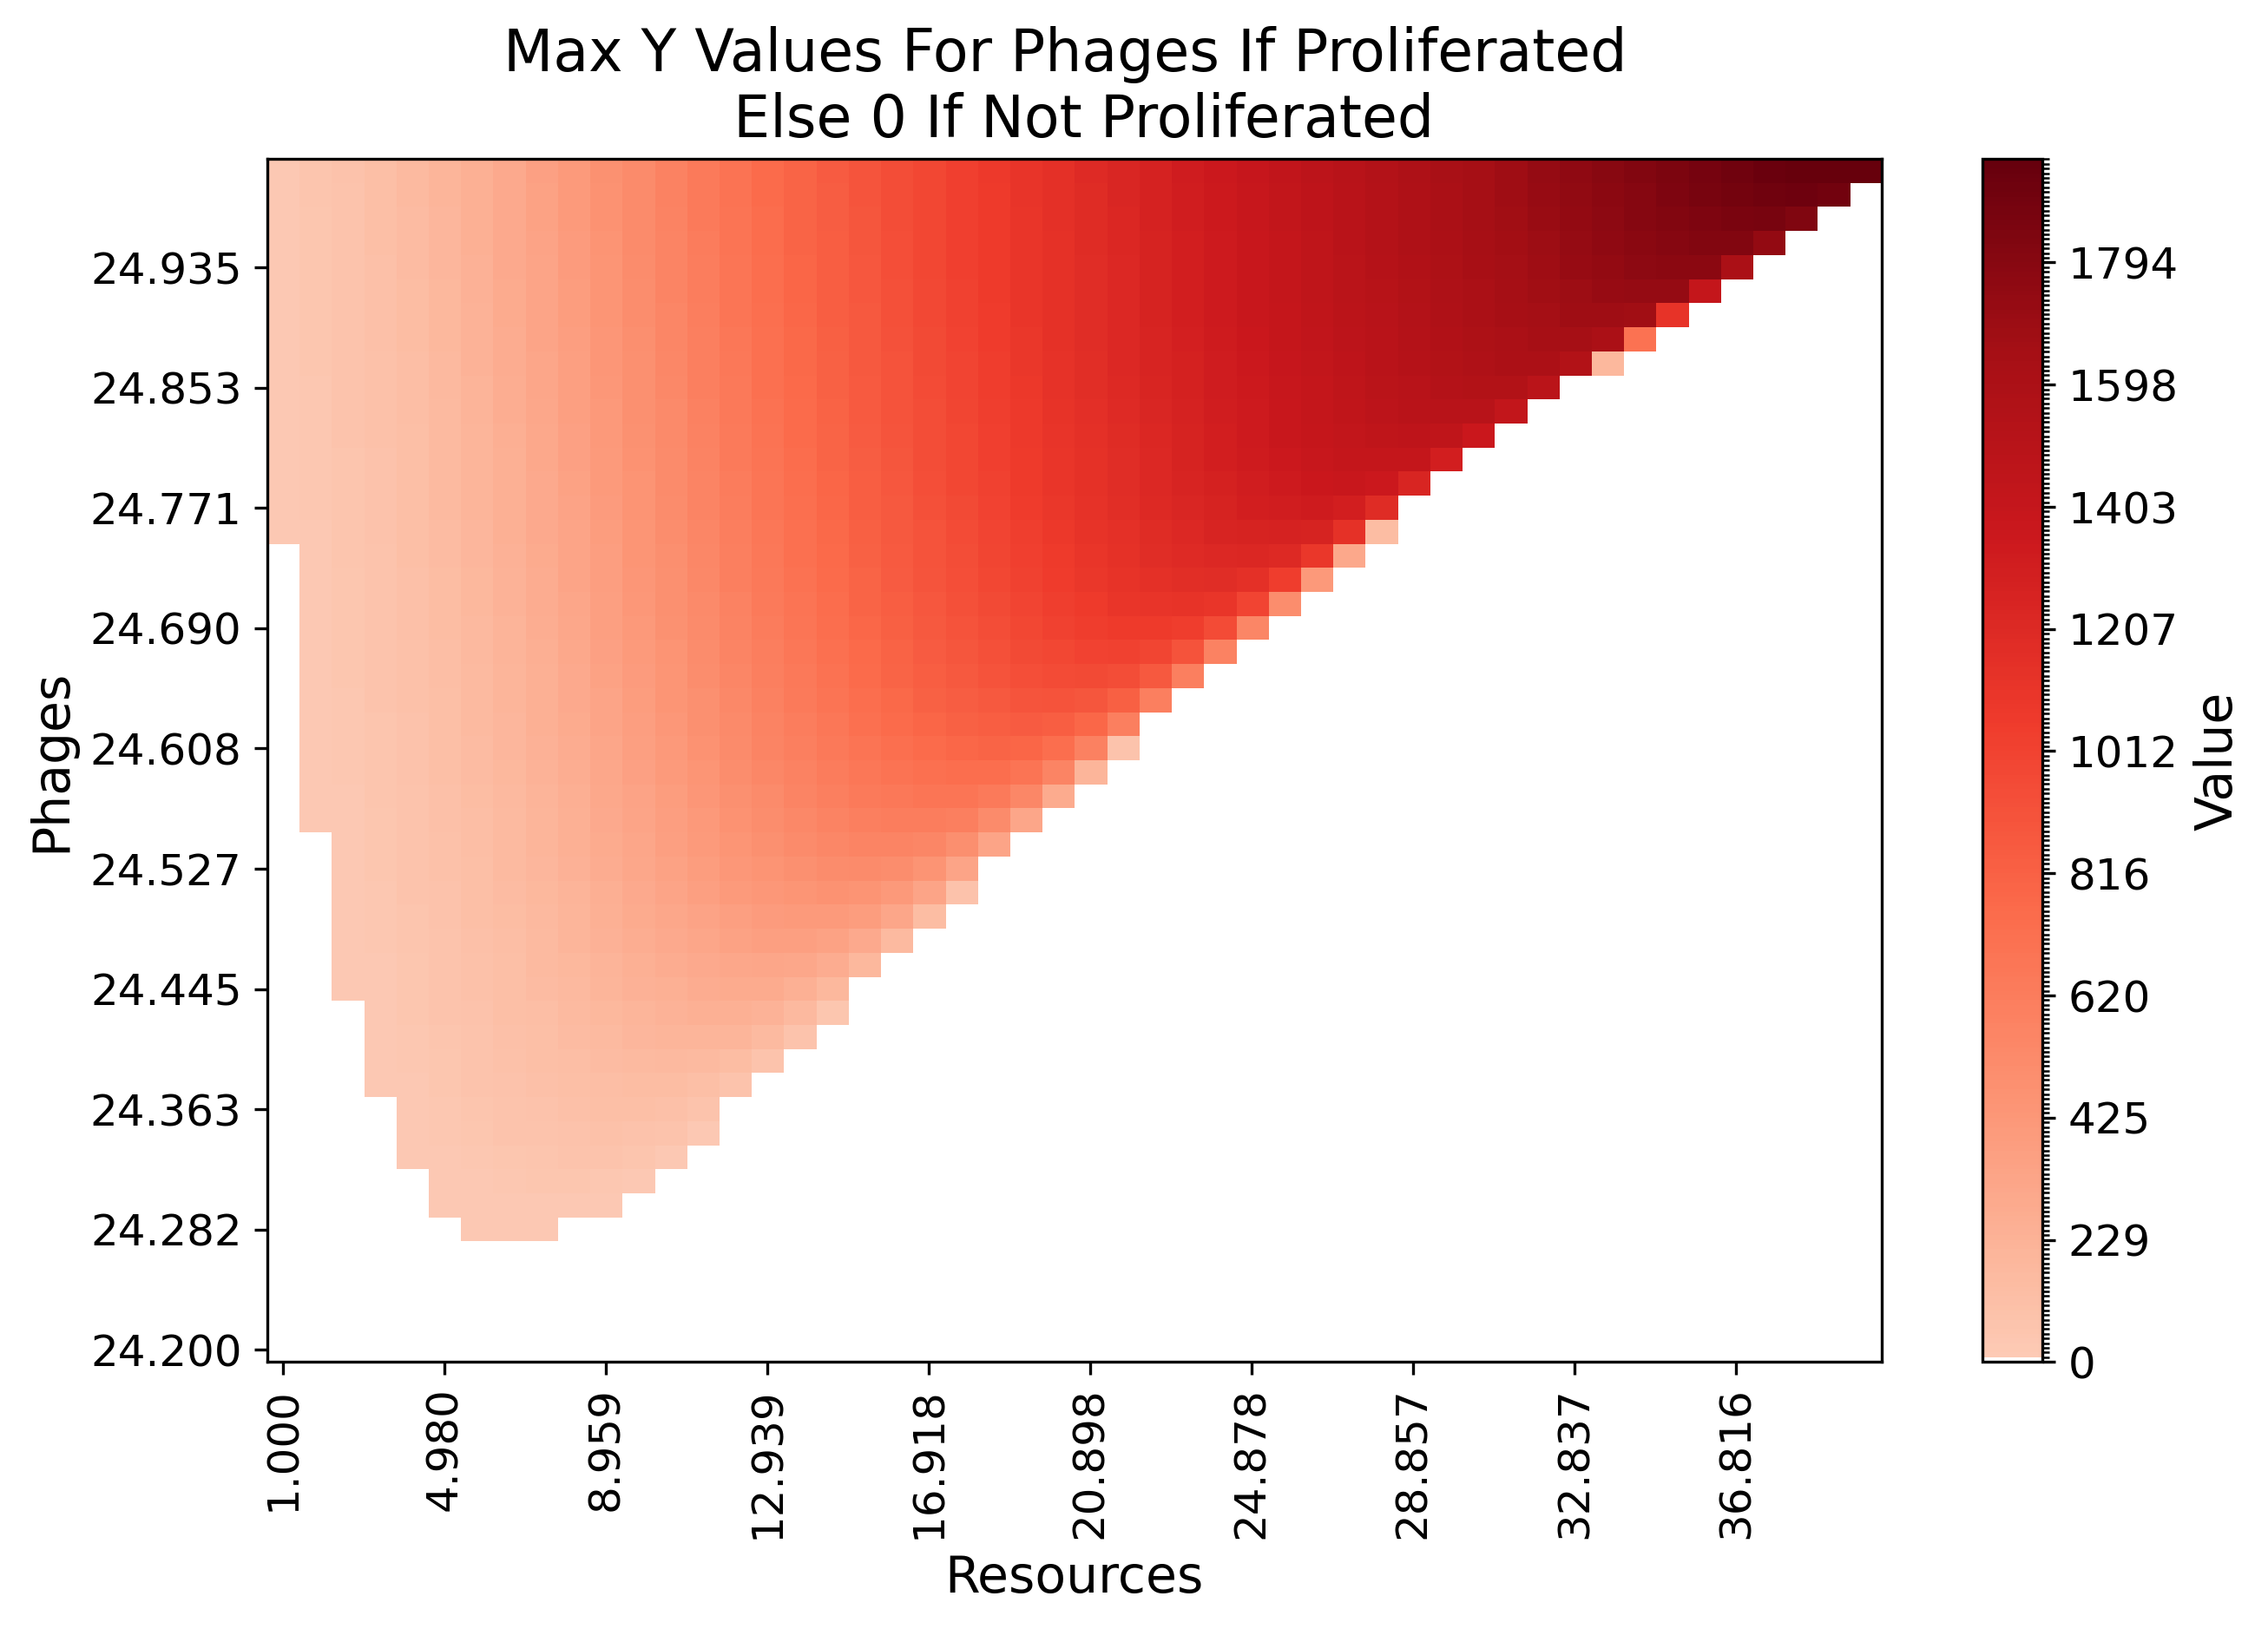
\includegraphics[width=\linewidth]{Plots/Created/PP/phase_portrait_resources_phage_2.png}
        \caption{
            Zoomed in to analyze the regime of behavior change near resources$=10$. 
        }
        \label{fig:created:phase_portrait_resources_phage_2}
    \end{subfigure}
    \caption{
        Varying initial resources and initial phages and the resulting proliferation and fitted proliferation curve. 
        The box is colored red if the phages proliferated for that condition, and white if the phages died out. 
        Phages proliferated if they reached 2 times their initial population at any point in time in the simulation. 
        This simulation used the values from \Cref{tab:appendixE:a_good_curve_2}, but with washout set to 0.02 instead of 0. 
    }
    \label{fig:created:phase_portrait_resource_phage_proliferate}
\end{figure}

\subsection{An Initial Phage, Bacteria, and Resource Analysis for Phage Proliferation}
The initial resource concentration had some, but very limited impact on if the initial phage concentration would affect if the phages proliferate. 
Within the context of the basic Golding model, the initial uninfected bacteria population is one of three parameters that a researcher can easily control, with the other two being the initial resource and initial phage. 
For low initial uninfected bacteria populations, it will be harder for the phages to proliferate. 
There is not enough bacteria to infect before the washout will remove the phages from the system. 
While for large initial uninfected bacteria populations it will be easier for the phages to proliferate such that the washout won't immediately wash the phages out. 
So I extend the initial resource and phage population analysis by adding a third dimension to the analysis, the initial uninfected bacteria population. 
The aim of adding the uninfected bacteria is to see how the initial uninfected bacteria will 1) affect if the phage can proliferate, and 2) affect the max population that the phages can reach. 

\Cref{fig:created:3D_phase_portrait} has three axes, the initial phage, resource, and bacteria population value. 
The initial uninfected bacteria did not have a significant impact on the 1) if the phages would proliferate, and 2) by how much the phages would proliferate. 
If spliced along the bacteria axis, there is little difference in the shape of the curve. 
It was expected that as the uninfected bacteria count would increase there would be significantly fewer phages that would be needed to ensure phage proliferation. 
However, there is not a significant change in if the phages proliferated and by how much. 

This suggests that under a washout situation, ensuring that there are enough phages is the most important factor to ensure that the phages are not washed out. 

\begin{figure}[ht!]
    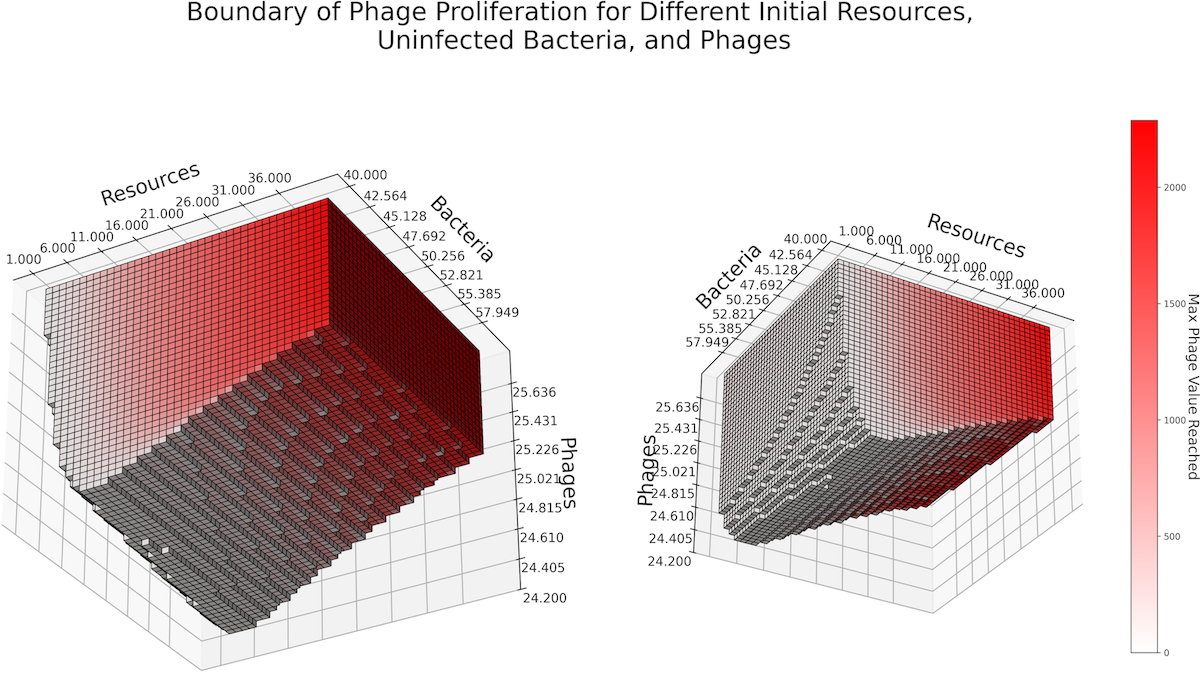
\includegraphics[width=1\textwidth]{Plots/Created/PP/3d_plot_resource_bacteria_phage.png}
    \centering
    \caption{
        3D plot of phage proliferation, dependent on initial resource, uninfected bacteria, and phage population. 
        Color scaling from white to red, color is dependent on the max phage population reached. 
    \label{fig:created:3D_phase_portrait}
    }
\end{figure}

\section{Plotting Parameter Change — $3\times 2\times 3$ Model}
Now that we have identified the most important parameters in the Golding model, we can analyze how the curve shapes change across a range of parameters for a larger model. 
The larger model will exhibit different behavior than a $1\times 1\times 1$ model due to the many interactions. 
The differing parameter values across each interaction will influence how fast each population can grow and die. 
A $3\times 2\times 3$ model was chosen as it is on the boundary between adding more phages, bacteria, or resources would clutter the plot with lines, while still offering behavior that can be compared against one another. 
The graph network that was used can be found at \Cref{fig:ss:example_network}, with the default parameter values found at \Cref{tab:appendixE:complex_model}. 
$B_0$ is infected by $P_1$ and $P_2$, and consumes $R_0$ and $R_1$. 
$B_1$ is infected by $P_0$ and $P_2$, while consuming $R_2$. 


\Cref{fig:created:r_beta_washout_0}, \Cref{fig:created:r_beta_washout_0.02}, and \Cref{fig:created:r_beta_washout_0.05}, show a $7\times7$ matrix of subfigures across washout rates of 0, 0.02, and 0.05
Each subfigure uses a different combination of $r$ and $\beta$ parameter values. 
However, we will specifically focus on \Cref{fig:created:r_beta_washout_original_original_0}, \Cref{fig:created:r_beta_washout_original_100_0}, and \Cref{fig:created:r_beta_washout_original_original_0.02}. 
All initial phage values started at 10. 
This was specifically chosen to show how even though the phage values all start the same, the different parameter values and interactions ultimately influence the population growth. 

If $r$ or $\beta$ is equal to $Original$, then the simulation uses the original parameter values as defined in \Cref{tab:appendixE:complex_model}, otherwise each $r$ and each $\beta$ parameter interaction has the value listed in the subfigure title. 

The columns and rows of each figure show how a change in parameter value affects the curve, while keeping the other parameter the same. 
In $r, \beta, \omega^o=Original, Original, 0$, although not a realistic growth curve, shows how the different parameter values for each interaction uniquely affect the growth rate of each entity, especially the phage population (P0=blue, P1=green, and P2=purple). 
Despite all phages starting at the same population level, within the first two or so time units, P1 has less phages than P0 and P2. 
P2 has the fastest initial growth rate, as P2 has the most phages until $t=4$, at which point P1 has a larger phage population. 
P2 reaches its peak population count before P0 or P1, but despite the slower initial growth, P0 and P1 eventually overtake P2 in total phage population. 
P2 also actually reaches its peak before decreasing in population. 
Since the phage population is reduced by $r_{pb}\cdot(U_b + \sum_{k=1}^M I_{b_k})$, and by specifically choosing the parameter values as used in \Cref{tab:appendixE:complex_model}, behavior that hasn't been seen in a $1\times 1\times 1$ system has been found. 
The complete extinction of the bacteria has been delayed long enough such that at trace amounts, there is phage reduction despite bacteria still existing. 
The peak times for P0, P1, and P2 are $t=6.33, 7.99, 4.52$, a difference of $3.47$ time units. 

Contrast that with the phage population dynamics of that with $r, \beta, \omega^o = Original, 100, 0$, the phage populations do not show interesting dynamics. 
The peak times are more similar and consistent to one another ($t=5.50, 7.01, 6.78$, a difference of $1.51$ time units). 
The phage population curve all appear the same, with slightly slower growth rates. 
There is no crossing of phage populations unlike with $r, \beta, \omega^o=Original, Original, 0$. 

The highlighted example demonstrated the dynamics and influence that multiple agents can have on the final output. 

The top row of \Cref{fig:created:r_beta_washout_0.02} shows how the phages and resources died out relative to the top row of \Cref{fig:created:r_beta_washout_0}. 
Even with a high burst value, the phages could not defeat the pressure from the washout. 
But by changing the $r$ value from $r=0.001$ to $r=0.041$, the phages were able to save themselves and proliferate. 


\begin{figure}[]
    \centering
    \begin{subfigure}{0.32\linewidth}
        \centering
        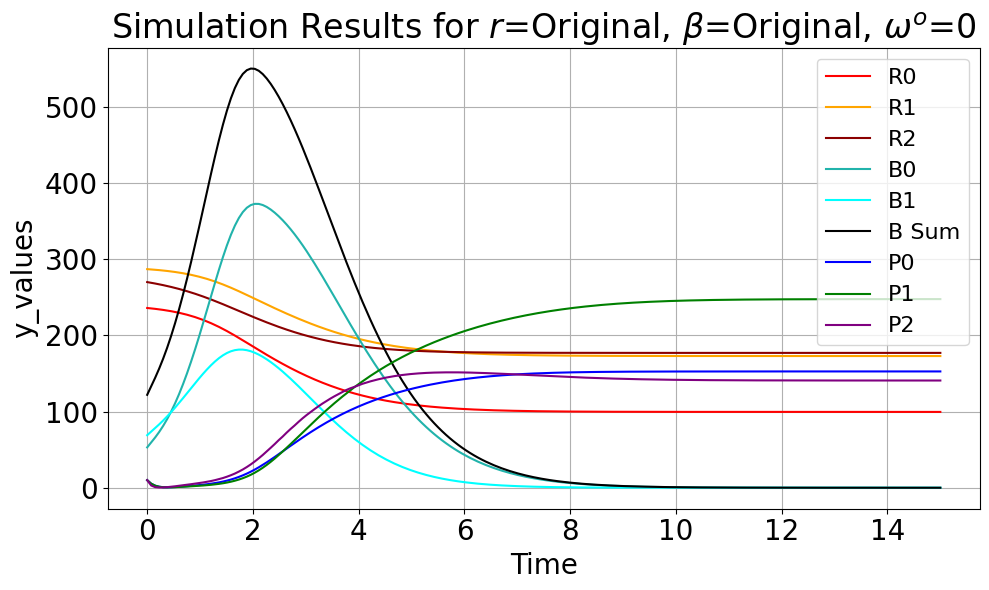
\includegraphics[width=\linewidth]{Images/Plots/Created/UA/r_beta_washout_Original_Original_0.png}
        \caption{
            $r, \beta, \omega^o = Original, Original, 0$, all initial phage condition=10. 
        }
        \label{fig:created:r_beta_washout_original_original_0}
    \end{subfigure}
    \begin{subfigure}{0.32\linewidth}
        \centering
        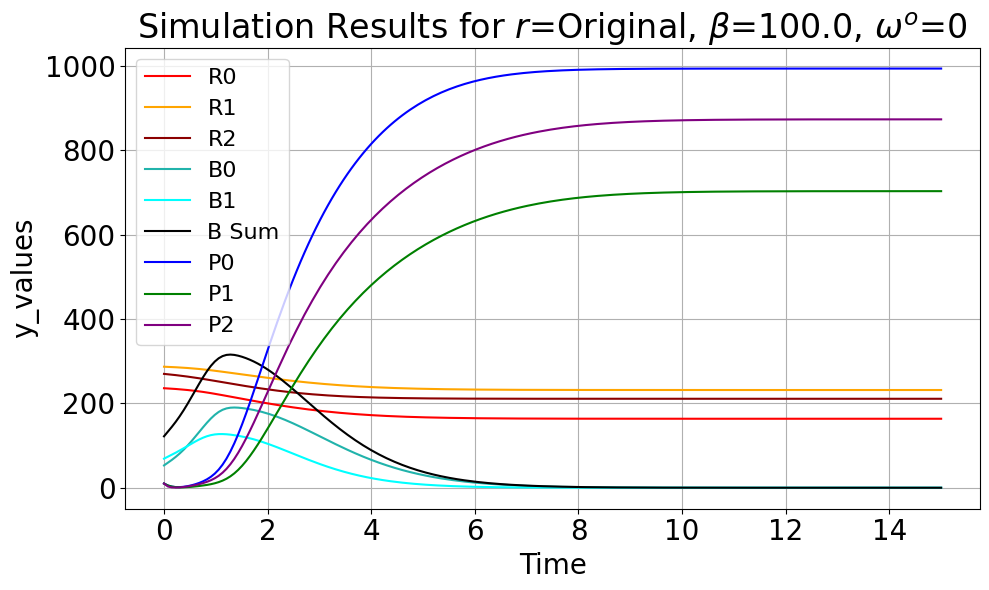
\includegraphics[width=\linewidth]{Images/Plots/Created/UA/r_beta_washout_Original_100.0_0.png}
        \caption{
            $r, \beta, \omega^o = Original, 100, 0$, all initial phage condition=10. 
        }
        \label{fig:created:r_beta_washout_original_100_0}
    \end{subfigure}
    \begin{subfigure}{0.32\linewidth}
        \centering
        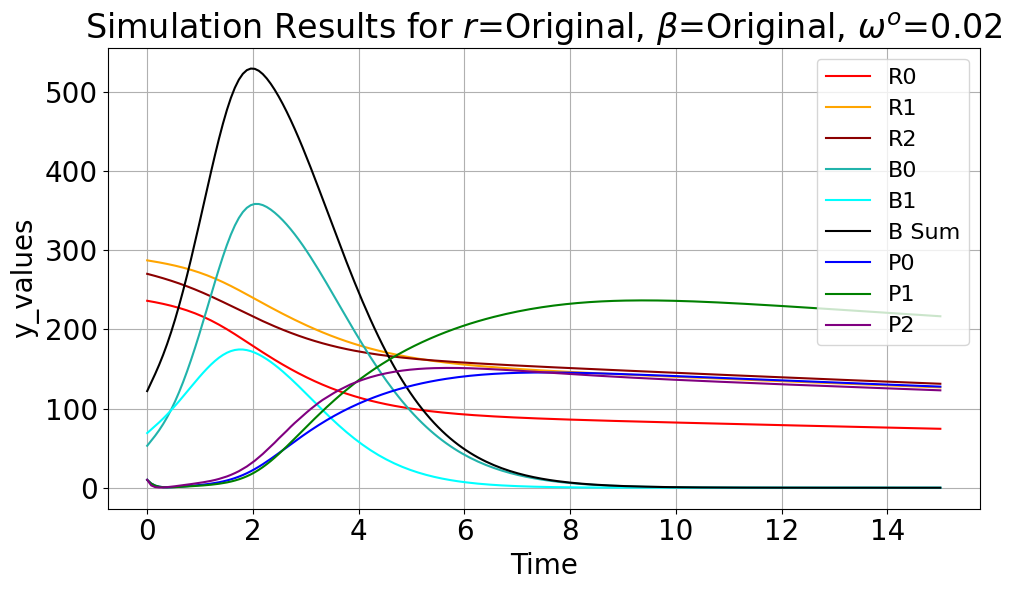
\includegraphics[width=\linewidth]{Images/Plots/Created/UA/r_beta_washout_Original_Original_0.02.png}
        \caption{
            $r, \beta, \omega^o = Original, Original, 0.02$, all initial phage condition=10. 
        }
        \label{fig:created:r_beta_washout_original_original_0.02}
    \end{subfigure}
    \caption{
        Varying $r$, $\beta$, and $\omega^o$. 
        All phage values set to 10 to show how the network connections and vector/matrix values affect phage growth. 
        Selectively chosen sub-figures from \Cref{fig:created:r_beta_washout_0}, \Cref{fig:created:r_beta_washout_0.02}, and \Cref{fig:created:r_beta_washout_0.05}. 
        Chosen parameter values can be found in \Cref{tab:appendixE:complex_model}. 
    }
    \label{fig:created:r_beta_washout}
\end{figure}

\section{Phage and Bacteria,Survivability Analysis For A $20\times20\times10$ System}
Using the simulation framework, I created and analyzed a $20\times20\times10$ system. 
I selected two parameters, $\tau$ and $\beta$, to run a survivability analysis using the extended Golding model. 
Each phage is guaranteed to interact with at least one bacterium but no more than two bacteria. 
Each bacterium interacts with at least one phage and one resource, but not more than two phages and two resources. 
Every resource interacts with at least one bacterium, and at most three bacteria. 
The parameter values were randomly selected from a uniform distribution in the SOBOL analysis value ranges (\Cref{tab:appendixE:SOBOL_analysis_values}). 
A phage survived if its final population is greater than 1 at the end of the simulation. 

\begin{figure}[]
    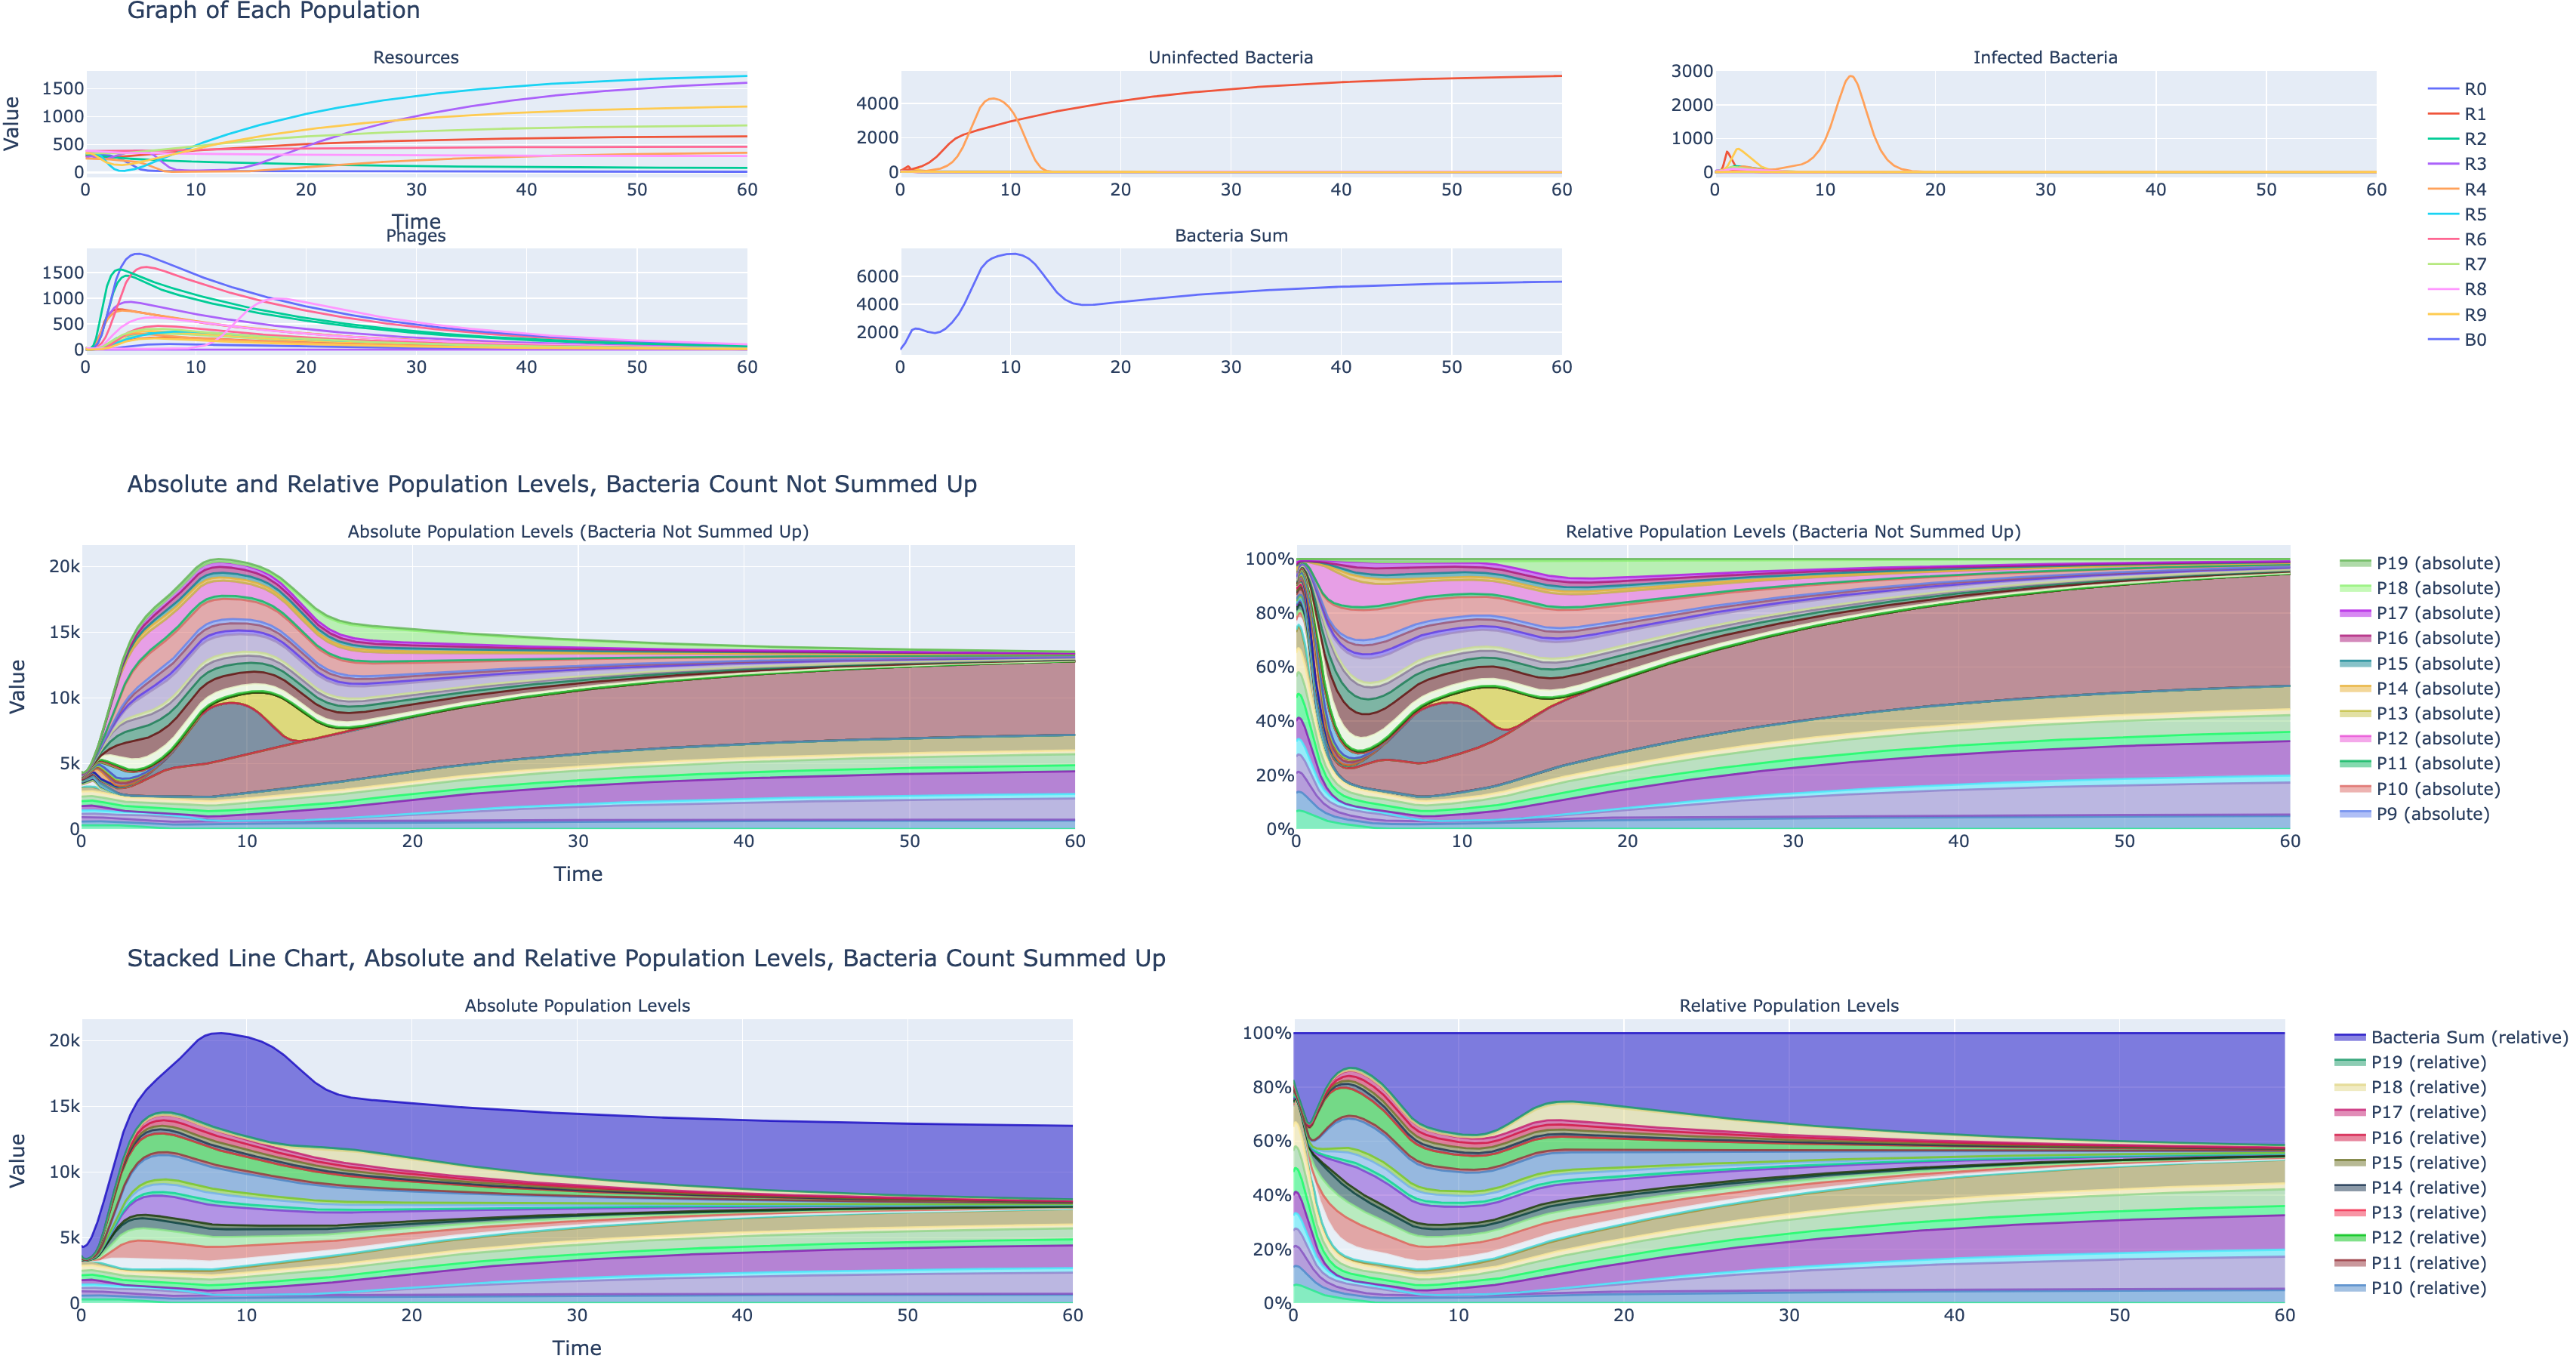
\includegraphics[width=1\textwidth]{Plots/Created/large_graph_output.png}
    \centering
    \caption{
        The output graph for the default parameter values for a large $20\times 20 \times 10$ network. 
        Parameter values were randomly chosen in the interval given by \Cref{tab:appendixE:SOBOL_analysis_values}. 
    \label{fig:created:large_graph_output}
    }
\end{figure}